\documentclass[pt, a5paper]{article}

\usepackage{hyperref}
% package below for jusifing
\usepackage{graphicx}
\usepackage{ragged2e}
\usepackage{color}
% persian lang
\usepackage{xepersian}
% persian lang font
\settextfont[Scale=1]{XB Roya}
% line height
\renewcommand{\baselinestretch}{1.5}

\begin{document}
\centerline{جزوه درس مدار منطقی}
\centerline{علیرضا سلطانی نشان}
\centerline{دانشجوی نرم افزار}
\centerline{ترم سوم}
%\date{\today}
\tableofcontents


\section{اعداد - مبناها - مکمل ها - کدها}

کلا اگه ما بخوایم هر عددی را نمایش بدهیم یا آنرا بنویسیم، این اعداد میتواند مبنا های مختلفی داشته باشد. در حالت کلی عددی مثل a را میتوانیم اینگونه نمایش دهیم:\\

\begin{itemize}\centering
	\item
		$a = a_{n-1} a_{n-2} ... a_2 a_1 a_{0}.a_{-1}a_{-2}a_{-3}...a_{-m}$
\end{itemize}


در حقیقت هر کدام از این اعداد دارای ارزش مکانی هستند، که در زیر به درستی نشان داده شده است :\newline

\begin{itemize}\centering
\item
$a = a_{n-1}^{^{r^{n-1}}},  a_{n-2} ^{^{r^{n-2}}},  
...  a_2 ^{^{r^{2}}}, a_1^{^{r^{1}}},  a_0^{^{r^{0}}}, . 
a_{-1}^{^{r^{-1}}},  a_{-2}^{^{r^{-2}}},  a_{-m}^{^{r^{-m}}}$
\end{itemize}


که بعد از اعشار (0) دارای n رقم عدد صحیح و قبل آن n رقم عدد اعشاری داریم.\\
نکته مهمی که در اینجا بایستی یادآوری شود آنست که هر عدد به توان منفی برابر است با:\newline

\begin{itemize}\centering
	\item
		$r^{-m} = \frac{1}{r^{m}}$
\end{itemize}



معرفی انواع مبنا ها:\newline
\begin{enumerate}\raggedright
	\item
	 $ 0...1 $ = {مبنای دو Binary}		
	\item
		 $ 0...9 $ = {مبنای 10 Decimal}		
	\item
	 $ 0...7 $ = {مبنای هشت Octal}		
	\item
	 $  0 ... 9 , A, B, C, D, E, F$ = {مبنای 16 Hexa Decimal}	
\end{enumerate}

 نکته: زمانی که در مبناها، به مبنا های بزرگی میرسیم، ما از 0 تا 9 را به رسمیت میدانیم و برای نمایش اعداد بعد از آن از حروف انگلیسی استفاده میکنیم.\\

اگر عددی در مبنای r باشد و بخواهیم آنرا به مبنای 10 تبدیل کنیم کافیست هر رقم را در ارزش مکانی خودش ضرب کرده و حاصل را باهم جمع کنیم.\newline


\subsection{تصاعد هندسی}
$(r - 1)_{_{_{r^{1}}}}(r - 1)_{_{_{r^{0}}}}.(r - 1)_{_{_{r^{-1}}}}(r - 1)_{_{_{r^{-m}}}} = (r - 1)\frac{r^{n}-1}{r-1} = r^{n}-1$\newline

بطوری که r مبنا و n تعداد ارقام است، بطور مثال، در مبنای دسیمال که سیستم دهدهی است، برای بدست آوردن بزرگ ترین عدد مجموعه از
$r - 1$
که میشود 9، یعنی 9 بزرگ ترین عدد مجموعه مبنای دسیمال است، و اگر به تعداد دو رقم آنرا در نظر بگيريم، يعنی 99، در جایگاه مربوطه بررسی خواهیم کرد، یعنی
$(10^{0} * 9) + (10^{1} * 9) = 99$
ودر مقابل تصاعد هندسی داریم،
$10^{2} - 1 = 99 $
.

\textbf{تمرین: تبدیل مبناهای زیر را انجام دهید:}
\newline

در هنگام انجام تبدیل مبنا های زیر، قصد یادآوری مطالب گذشته است، اما در بین آنها مطابی هم ذکر شده است که نکاتی را در بر دارند و بایستی به عنوان مطلب جدید آنرا در نظر داشت:\\

\textbf{نکات}\\

برای تبدیل مبنا از 10 به هر مبنای دیگری باید 10 را در آن مبنا پی در پی تقسیم کنیم که در نهایت به با استفاده از باقی مانده ها و مقسوم علیه آخر تقیسم از راست به چپ نتایج تقسیم را کنار هم بگذاریم.\\

در هنگام تبدیل مبنا، جلوترین و اخرین ارزش مکانی عدد را MSB یا
$ Most  Significant Bit$
و کمترین و اخرین ارزش مکانی در عدد را LSB یا
$Least Significant Bit$
 گفته میشود. مانند: $(327.2)_{10}$ که عدد 3 $MSB$ و 7 
$ LSB$
 .\newline
 

\subsection{تبدیل مبنا از 2 به 10 یا بلعکس}
در تبدیل مبنا از 2 به 10 میبایست به صورت عادی با استفاده از ارزش مکانی هر عدد
$2^{0}$
و
$2^{1}$
و...
یا به صورت خودمان
1, 2, 4, 8, 16, 32, 64,...
و در نهایت هر قسمتی که بیت روشن یا 1 داشت را نتیجه را با هم جمع میکنیم.\\
\subsection{تبدیل مبنا از 2 به 10}
تمرین: \\
\begin{itemize}\raggedright
	\item
		$(11001)_{2_{\rightarrow 10}} = (1*1)+(1*8)+(1*16) = 1+8+16 = 25$
		
	\item
		$(1111001)_{2_{\rightarrow 10}} = (1*1) + (1*8) + (1*16) + (1*32) + (1*64) = 1 + 8 + 16 + 32 + 64 = (121)_{10}$
		
	\item 
	$(100011111)_{2_{\rightarrow 10}} = (1*1) + (1*2) + (1*4) + (1*8) + 1*16) + (1*256) = (281)_{10}$ 
\end{itemize}
\subsection{تبدیل مبنا از 10 به دو}
همانطور که در بالاتر گفته شد در تبدیل مبنا از 10 به 2 یا به هر مبنای دیگر میتوانیم هب راحتی از تقسیم پی در پی 10 در مبانی مورد نظر با استفاده از باقی مانده ها به جواب نهایی برسیم.\\
تمرین: \\
\begin{itemize}\raggedright
	\item
	$(34)_{10_{\rightarrow 2}} = $
	\begin{table}[ht] \raggedright
		\begin{LTR}
			\begin{tabular}{| c | c |}
				\hline
				Calculate & باقی مانده\\
				34 / 2 = 17 & 0 \\
				17 / 2 = 8  & 1 \\
				8 / 2 = 4   & 0 \\
				4 / 2 = 2   & 0 \\
				2 / 2 = 1   & 0 \\
				1 / 2 =     & 1 \\
				\hline
			\end{tabular}
		\end{LTR}
	\end{table}
	$(34)_{10_{\rightarrow 2}} = 100010$
			
\end{itemize}

\subsection{تبدیل مبنا از 10 به هشت و برعکس}

\begin{itemize}
\item
	$(972)_{10_{\rightarrow 8}} = $
	\begin{table}[ht] \raggedright
		\begin{LTR}
			\begin{tabular}{| c | c |}
				\hline
				Calculate & باقی مانده\\
				972 / 8 = 115 & 7 \\
				115 / 8 = 14  & 3 \\
				14 / 8 = 1    & 6 \\
				1 / 8 = 0     & 1 \\
				\hline
			\end{tabular}
		\end{LTR}
	\end{table}
	$(972)_{10_{\rightarrow 8}} = (1637)_{8}$
	
	\item
	$(1637)_{8_{\rightarrow 10}} = (7 * 8^{0}) + (3 * 8^{1}) + (6 * 8^{2})+ (1 * 8^{3})= (927)_{10}$
\end{itemize}


\subsection{تبدیل اعداد صحیح از مبنای 10 به 16 و برعکس}
برای تبدیل مبنا از 10 به 16 درست مثل قبل از تقسیم پیا پی 10 در 16 استفاده خواهیم کرد:\\

\begin{itemize}
	\item
	$(954)_{10_{\rightarrow 16}}$
	\begin{table}[ht] \raggedright
		\begin{LTR}
			\begin{tabular}{| c | c |}
				\hline
				Calculate & باقی مانده\\
				954  / 16 = 59 & 10$\rightarrow$ A \\
				59  / 16 = 3   & 11$\rightarrow$ B \\
				3  / 16   = 0  & 3 \\
				\hline
			\end{tabular}
		\end{LTR}
	\end{table}
	$(954)_{10_{\rightarrow 16}} = (3BA)_{16}$	
	
	\item
	$(3BA)_{16_{\rightarrow 10}} = (10 * 16^{0}) + (11 * 16^{1}) + (3 * 16^{2}) = 954 $	
\end{itemize}



\subsection{تبدیل اعشاری دهدهی به دودویی و برعکس}
مهم ترین بخش تبدیل مبناها زمانیست که شما با مبنایی اعشاری رو به رو میشوید، در حالت تبدیل مبنا از دودویی به سیستم دهدهی، قسمتی که به صورت صحیح است را طبق معمول محاسبه می کنیم، و آن قسمتی که بعد از اعشار قرار دارد، به صورت
$2^{-1}, 2^{-2}, 2^{-3}... $
محاسبه خوهیم کرد و در نهایت نتیحه قسمت صحیح را به نتیجه قسمت اعشاری قرار خواهیم داد:\\

\begin{enumerate}\raggedright
	\item
	$(1110.01)_{2 \rightarrow 10} = $\\
	$(1110)_{2 \rightarrow 10} =  14$\\
	$(.01)_{2 \rightarrow 10} = (0 * 2^{-1}) + (1 * 2^{-2}) = \frac{1}{4}$\\
	$\rightarrow 14 + \frac{1}{4} = \frac{56}{4} + \frac{1}{4} = \frac{57}{4} = 14.25$	

	\item
	$(10111001.0101)_{2 \rightarrow 10} = $\\
	$(10111001)_{2 \rightarrow 10} = 185$\\
	$(0.0101)_{2 \rightarrow 10} = \frac{1}{4} + \frac{1}{16} = \frac{4}{16} + \frac{1}{16} = \frac{5}{16} = 0.3125$\\
	$\rightarrow 185 + 0.3125 = 185.3125$\\
	
\end{enumerate}

حلا نوبت به انجام تبدیل مبنا 10 به 2 میرسد، در این بخش، طبق معمول آن قسمتی که سمت صحیح عدد قرار دارد را به صورت عادی از 10 به 2 تبدیل میکنیم، اما آن بخشی که به صورت اعشاری است را باید کمی توجه کنیم، قسمت اعشاری را ضرب 2 میکنیم، و حاصل آن را بررسی میکنیم و قسمت صحیح حاصل را به عنوان نتیجه تقسیم اول در نظر میگیرم، و آن بخش اعشاری را (فقط اعشاری) دو باره ضرب در دو میکنیم، انقدر این ضرب را انجام میدهیم که قسمت اعشاری به صفر برسد، ممکن است در طی این عملیات تعداد ضرب کردن به 2 زیاد شود، در این مواقع تا هشت مرحله ضرب کردن کافی است (قاعده پرشدن حافظه 8 بیت). لازم به ذکر است که در تمامی تبدیل های سیستم دهدهی به هر مبنای دیگیری، مانند باینری یا اکتال یا سه سه ای، چهارچهاری و غیره دقیقا همان عملیاتی که گفته شد صورت میگیرد، هم بخش تقسیم پیاپی در قسمت صحیح، هم ضرب متناوب در قسمت اعشاری.\\

تمرین: \\
\begin{enumerate}\raggedright
	\item
	$(12.25)_{10 \rightarrow 2} = $\\
	$(12)_{10 \rightarrow 2} = (1100)_{2}$\\
	$(0.25)_{10 \rightarrow 2} = $\\	

	\begin{table}[ht] \raggedright
		\begin{LTR}
			\begin{tabular}{| c | c |}
				\hline
					0.25 * 2 = 0.5 & 0\\
					0.5 * 2 = 1.0  & 1	\\			
				\hline
			\end{tabular}
		\end{LTR}
	\end{table}		
	\raggedleft
بعد از اینکه عدد اعشار حاصل دومین ضرب برابر با صفر شد دیگر نیازی به ضرب کردن نیست و از همان دو عدد نتیجه 0 و 1 استفاده میکنیم و در نتیجه خواهیم داشت:\\
	$\rightarrow (1100.01)$\raggedright

	\item
	$(15.361)_{10 \rightarrow 2} = $\\
	$(15)_{10 \rightarrow 2} = (1111)_{2}$\\
	$(0.361)_{10 \rightarrow 2} = $\\	

	\begin{table}[ht] \raggedright
		\begin{LTR}
			\begin{tabular}{| c | c |}
				\hline
					0.361 * 2 = 0.722 & 0\\
					0.722 * 2 = 1.444  & 1	\\			
					0.444 * 2 = 0.888  & 0	\\
					0.888 * 2 = 1.776  & 1	\\
					0.776 * 2 = 1.552  & 1	\\
					0.552 * 2 = 1.104  & 1	\\
					0.104 * 2 = 0.208  & 0	\\
					0.208 * 2 = 0.416  & 0	\\
				\hline
			\end{tabular}
		\end{LTR}
	\end{table}
			
	\raggedleft
	$\rightarrow (1111.01011100)$\raggedright
\end{enumerate}

\subsection{تبدیل اعداد مبنای دو به مبنای هشت و برعکس}
برای تبدیل مبنای دو به هشت فقط کافی است از سمت راست به چپ سه بیت سه بیت جدا کنیم و براساس ریتم 1، 2، 4 آنها را باهم جمع کنیم، نکته ای که در این میان باید توجه کنیم ان است که اگر تعداد ارقام مضربی از سه نباشد، بایستی از سمت چپ، عدد صفر اضافه کنیم.\\

مثال/تمرین: \\

\begin{enumerate}\raggedright
	\item
	$(11001)_{2 \rightarrow 8} = $\\
	$(011'001)_{2 \rightarrow 8} = (31)_{8} $\\

	\item
	$(1110001)_{2 \rightarrow 8} = $\\
	$(001'110'001)_{2 \rightarrow 8} = (161)_{8}$\\	
	
	\item 
	$(100111)_{2 \rightarrow 8} = $\\
	$(100'111)_{2 \rightarrow 8} = (47)_{8}$\\	
\end{enumerate}

تبدیل مبنا اعشاری از دو به هشت:\\
این نوع تبدیل مبناهم بایستی در نظر داشته باشیم که بهتر به دوقسمت صحیح و اعشاری تقسیم می شود، در قسمت اعشاری اگه تعداد ارقام مضربی از 3 بود میتوان به صورت سه تا سه از راست به چپ ازجدایی را انجام داد، در غیر این صورت باید از سمت چپ به تعداد لازم 0 اضافه کنیم. در قسمت اعشاری هم همین قاعده صادق است، با این تفاوت که اگه تعداد ارقام سمت اعشار مضربی از 3 نبود این بار بایسیتی از سمت راست به تعداد لازم صفر وارد کنیم.\\

\begin{enumerate}\raggedright
	\item
	$(10011.1101)_{2 \rightarrow 8} = $\\
	$(010'011)_{2 \rightarrow 8} = (23)_{8} $\\
	$(0.110'100)_{2 \rightarrow 8} = (64)_{8} $\\
	$\rightarrow (23.64)_{8} $\\
\end{enumerate}

تبدیل برعکس 8 به 2 هم دقیقا به همین صورت است.

\begin{enumerate}\raggedright
	\item
	$(10101.0111)_{2 \rightarrow 8} = $\\
	$(010'101)_{2 \rightarrow 8} = (25)_{8} $\\
	$(011'100)_{2 \rightarrow 8} = (34)_{8} $\\
	$\rightarrow (25.34)_{8} $\\
	
	\item
	$(25.34)_{2 \rightarrow 8} = $\\
	$(010'101)_{2 \rightarrow 8} = (25)_{8} $\\
	$(011'100)_{2 \rightarrow 8} = (34)_{8} $\\
	$\rightarrow (10101.0111)_{2} $\\
	
	\item
	$(55.67)_{2 \rightarrow 8} = $\\
	$(101'101)_{2 \rightarrow 8} = (55)_{8} $\\
	$(110'111)_{2 \rightarrow 8} = (67)_{8} $\\
	$\rightarrow (101101.110111)_{2} $\\
	
\end{enumerate}

\subsection{تبدیل مبنا 2 به 16 و برعکس}
در تبدیل مبنا از 2 به 16 هم دقیقا مانند مبنای 8 است که، بطوری که باید تعداد ارقام ضریبی از 4 باشند و در هنگام اعشاری شدن هم باید برای جبران کسری صفر در سمت چپ برای عدد صحیح و در سمت راست برای عدد اعشاری.\\


\begin{enumerate}\raggedright
	\item
	$(1111101)_{2 \rightarrow 16} = $\\
	$(0111'1101)_{2 \rightarrow 16} = (7D)_{16} $\\
	
	
	\item
	$(1011101100)_{2 \rightarrow 16} = $\\
	$(0010'1110'1100)_{2 \rightarrow 16} = (2EC)_{16} $\\
	
	\item 
	Decimal 2 to 16
	$(1111101.0110)_{2 \rightarrow 16} = $\\
	$(0111'1101)_{2 \rightarrow 16} = (7D)_{16} $\\	
	$(.0110)_{2 \rightarrow 16} = 6$\\	
	$\rightarrow (7D.6)_{16}$ 
	
	\item 
	16 to 2
	$(F25.03)_{16 \rightarrow 2} = $\\
	$(F25)_{16 \rightarrow 2} = (1111'0010'0101)_{2}$\\
	$(.03)_{16 \rightarrow 2} = (0000'0011)_{2}$\\
	$\rightarrow (111100100101.00000011)_{2}$ 
\end{enumerate}


\subsection{تبدیل اعداد مبنای 8 به 16 و برعکس}


\begin{enumerate}\raggedright
	\item
	$(A36)_{16 \rightarrow 8} = $\\
	$(1010'0011'0110)_{16 \rightarrow 2} = (101000110110)_{2} $\\
	$(101'000'110'110)_{2 \rightarrow 8} = (5066)_{8} $\\
	
	\item
	$(753)_{8 \rightarrow 16} = $\\
	$(111'101'011)_{8 \rightarrow 2} = (111101011)_{2} $\\
	$(0001'1110'1011)_{2 \rightarrow 16} = (1EB)_{16} $\\
\end{enumerate}

\textbf{Extra}\\
ممکن است بخواهيم از عددی که به صورت دسیمال است متوجه بشویم که این عدد در مبنای دو چند بیتی است، برای این کار، چون که در مبنای دو هستیم، پس بر پایه توانی از 2 پیش میرویم، به همین خاطر عددی که بدست خواهید آورد بایستی از عدد دسیمال گفته شده بزرگ تر مساوری باشد. مانند:\\

\begin{LTR}
	$(768)_{10 \rightarrow 2}$\\
	$2^{8} = 256 -1 >= 768$\\
	$2^{9} = 512 -1 >= 768$\\
	$2^{10} = 1024 -1 >= 768$\\	
\end{LTR}

پس متوجه خواهید شد که عدد 768 وقتی به بانیتری تبدیل میشود 19 بیتی خواهد بود.


\subsection{متمم ها یا (Complements)}

متمم ها در کامپیوتر های دیجیتال برای ساده کردن عمل تفریق و یا عملیات منطقی به کار میروند. ساده سازی عملیات منجر به پیاده سازی مدارات ساده تر میگردد. در هر مبنایی مانند r، دو نوع متتم وجود دارد: یکی متمم مبنا و دیگری متمم کاهش یافته. فرم اول به نام متتم r و دومی به متمم
$r - 1$
مرسوم است. وقتی که مقدار مبنا(یا پایه) را جایگذین کنیم، برای اعداد دودویی، متمم ها ی2 و 1 و برای دهدهی، متمم های 10 و 9 را خواهیم داشت.

\textbf{دو نوع متتم برای هر عدد در مبنای r وجود دارد:}
\begin{itemize}
	\item
متمم مبنا یا مکمل r
	\item
	متمم مبنای کاهش یافته یا مکمل $r - 1$
\end{itemize}

اگر عدد N در مبنای r شامل n رقم باشد:\\
\begin{itemize}
	\item
	 متمم مبنا
	 $r^{n}-N$
	\item
	متمم مبنای کاهش یافته
	$(r^{n} - 1) - N$
\end{itemize}



\textbf{نکته بسیار مهم:}
$r^{n}$
در هر مبنایی برابر است با
$1+n(0)$\\

\raggedleft
\justifying
برای مثال در
$16^{3}$
درست است که برابر با 4096 میشود اما این عدد بدست آمده در واقع در مبنای 10 است نه در مبنای 16، بهمین خاطر بایستی عدد حاصله را در مبنای 16 تبدیل کنیم، که با توجه به قاعده بالا ما خواهیم داشت یک عدد 1 به همراه تعداد ارقام صفر یعنی 1000\\

$16^{3} = (1000)_{16}$
$8^{3} = 1000_{8}$
$10^{3} = 1000_{10}$
$2^{3} = 1000$\\

\justifying
اما، باید توجه داشته باشیم که هر کدام از اعداد بدست آمده بالا در حقیقت آنچیزی که نشان میدهد، نیست، فقط عدد 1000 در مبنای 10 است، که حقیقتا برابر این مقدار است، بقیه حالت ها در حالت ماکسیموم خود قرار دارند، یعنی 1000 در مبنای 8 برابر با 777 است.\\
و به یاد داشته باشید که در بدست اوردن مبنایی مانند 8 و هر مبنایی به غیر از 2 و 10 (برای مثال در اینجا هشت آورده شده)، مقدار 777 درواقع مقدار متمم کاهش یافته را به شما بر میگرداند.\\
و همچنین در این مبنا یعنی مبنای8، همانطور که گفته شد با 777 شما مکمل کاهش یافته را بدست خواهید آورد، برای بدست آوردن مکمل یا متمم 8 بایستی در نظر داشته باشید اگر عدد مبنای هشت شما در انتها دارای صفر بود، مانند 120، 40300، یا هر عددی که به تعداد صفر ختم شده باشد، در جواب این مسئله با تعداد عدد 7 در اخر عدد مواجه میشوید، برای داشتن متمم مبنای 8 همین تعداد 7 پایانی را کافیست برابر با صفر قرار دهیم و یک عدد به عدد بعد از آن اضافه کنیم\\
لازم به ذکر است که در هر مبنایی به غیر از 10 و دو در بدست آوردن متمم ها، شما همیشه متمم کاهش یافته را بدست می آورید!\\
مثال های مهم برای این نکته:\raggedleft
\raggedright

$(123)_8 = 8^{3} - 123 = 777 - 123 = 654 reduce. 654 + 1 = 655 radix$\\
$(1230)_8 = 8^{3} - 1230 = 7777 - 1230 = 6547 reduce. 6547. 6540 + (4+1) \rightarrow 6550 $\\
\justifying
این مورد تنها در مبنای 8 نیست بلکه در مبناهای طبیعی دیگر، مانند 3، 4، 5، ... نیز وجود دارد.\\
\textbf{نتیجه گیری نهایی}
اگر، مبنای 10 دادن برای مکمل و مکمل کاهش، از قاعده بومی
$r^{n}-n$
و
$(r^{n}-1)-n$
استفاده میکنیم که مبنا به توان تعداد ارقام برابر با همان 1 با تعدادی صفر در جلوش است. در مبنای دو هم که طبق تعریف نیازی به دوباره کاری نیست، و فقط به قاعده ای که در چند خط بالا گفته شد دقت کنید.

\textbf{متمم اعداد}\\
\raggedleft
متمم 10 عدد 546700 برابر است با\\
\raggedright
$10^{6} - 546700 = 453300$\\ 
\raggedleft
متمم 9 عدد 546700 برابر است با\\
\raggedright
$(10^{6} - 1) - 546700 = 453299$\\
\raggedleft
روش سریع دیگر آن است که اگر به ما مبنا را دادند میتوانیم با یکی کم کردن از آن به مبنای کاهش یافته آن برسیم، و برعکس، اگر متمم مبنای کاهش یافته را به ما دهند میتوانیم با یکی اضافه کردن به آن به متمم مبنا برسیم!\\

متمم 2 عدد 1101100 برابر است با:\\
\raggedright
1101100 = 108\\
$2^{7} - 108 = (20)_{10} = (10100)_{2}$\\
\raggedleft
متمم 1 عدد 1101100 برابر است با:\\
\raggedright
$(2^{7} - 1) - 108 = (19)_{10 \rightarrow 2} = (0010011)_{2}$\\
\raggedleft
\textbf{متمم اعداد در مبنای 2 به سریع ترین روش}\\
\textbf{نکات}\\
متمم1: تمام ارقال NOT میشود.
متمم 2: تمام صفر های سمت راست تا زمانی که به اولین یک از سمت راست برسیم همان طور به شکل اول خود باقی می ماند، اما از آن به بعد بیت های بعدی NOT میشود.\\
متمم 1 عدد 0011011 برابر  است با: 1100100\\
متمم 2 عدد 1101100 برابر است با: 0010100\\

\textbf{این همه گفتیم، پس در سیستم 16 تایی چطوره؟}\\
برای بدست آوردن مکمل 16 و مکمل کاهشی آن (15) بایستی بدانیم که ماکسیموم برای n رقم مثل
$16^{3} = (1000)_{16}$
اخرین درجه برای مقدار 1000، 15 15 15 است که میبایستی این عدد را از  مبنای 16 کم کنیم تا آنگاه مبنای کاهش یافته را بدست بیاوریم.\\
مثال\\
\centering$(A86)_{16} = 16^{3} = 1000_{16} - A86 = 15 15 15 - 10 8 6 = 5 7 9 Reduce...579 (9+1=10=A)= 57 10 or 57A$

\textbf{تمرین}\\ \raggedleft

\begin{enumerate}\raggedleft
	\item
	مبنا 10 و مکمل 9 عدد
$(256.73)_{10}$
را بنویسید.\\

	\item
	
مبنا 10 و مکمل 9 عدد
$(325.12)_{10}$
را بنویسید.\\

	\item
	
هر دو مقدار 9 و 10
$(256.73)_{10}$\\
	\item
	
هر دو مقدار 9 و 10
$(325.12)_{10}$\\
	\item
	
هر دو مقدار 7 و 8
$(276.35)_{8}$\\

	\item
	
هر دو مقدار 9 و 10
$(9300)_{10}$\\
	\item
	
$(304000)_{8}$\\

	\item
	
$(11110100)_{2} = 00001100$\\
\end{enumerate}

\subsection{اعداد علامت دار}
اعداد را میتوان به 4 روش نمایش داد:\\

\begin{itemize}\raggedleft
	\item
	روش بدون علامت:\\
	عدد را به صورت عادی ارزش گذاری میکنیم و در نهایت نتیجه را مینویسیم
	\item
	روش مقدار علامت:\\
	سمت چپ ترین بیت نشان دهنده علامت عدد است.
	\item
	نمایش عدد به صورت مکمل یک
	\item
	نمایش عدد بصورت مکمل 2
\end{itemize}

\textbf{نکته}\\
\begin{itemize}\raggedleft
	\item
	در روش مقدار علامت، بیت صفر نشان دهنده مثبت بودن و بیت یک نشان دهنده منفی بودن است.
	\item
در مکمل یک عدد را به صورت مکمل یک نمایش میدهیم.
	\item
در مکمل 2 عدد را بصورت مکمل دو نمایش میدهیم.
\end{itemize}

\textbf{مثال}\\
عدد 8 بیتی
$(10010100)_{2}$
راب به مبنای دهدهی تبدیل کنید با فرض اینکه:\\

\begin{enumerate}\raggedleft
	\item
		این عدد در سیستم بی علامت باشد.
		$(10010100)_{2} = 4+16+128 = 148$
	\item
	این عدد در سیستم علامت مقدار باشد.
	$(10010100)_{2} = -(4+16) = -20$
	\item
	این عدد در سیستم مکمل 1 باشد.
	$(10010100)_{2} = -(01101011) = -(1+2+8+32+64)= -107 = $
	\item
	این عدد در سیستم مکمل 2 باشد.
	$(10010100)_{2} = -(01101100) = -(4+8+32+64) = -108 $
\end{enumerate}


\textbf{مثال}\\
عدد 8 بیتی
$(01000101)_{2}$
راب به مبنای دهدهی تبدیل کنید با فرض اینکه:\\

\begin{enumerate}\raggedleft
	\item
		این عدد در سیستم بی علامت باشد.
		$(01000101)_{2} = 69$
	\item
	این عدد در سیستم علامت مقدار باشد.
	$(01000101)_{2} = +69$
	\item
	این عدد در سیستم مکمل 1 باشد.
	$(01000101)_{2} = +(10111010) = 2+8+16+32+128 = +186$
	\item
	این عدد در سیستم مکمل 2 باشد.
	$(01000101)_{2} = +(10111011) = +187 $
\end{enumerate}

\raggedright
\justifying
\textbf{نکته مهم}\\
گاهی ممکن است بخواهیم عددی را منفی اش را به صورت دودویی بنویسیم اما باید یک نکته مهمی را مورد نظر داشته باشیم، برای مثال اگر از ما بخواهند که عدد 9 را نمایش دهیم آن را به صورت
$(1001)_{2}$
نشان میدهیم، اما اگر از ما بخواهند که منفی این عدد را نمایش بدهیم نمی توان آنرا به این صورت
$(11001)_{2}$
نشان داد، در حقیقت بازهم به جواب 9- خواهیم رسید اما در 5 بیت معنایی ندارد، چرا که کامپیوتر همه اعداد در در تعدادی از توان های دو نمایش میدهد مانند 4 بیت، 8 بیت، 16، 32، 64، 128 و غیره. پس برای نشان دادن عدد -9 باید به این صورت بنویسیم:
$({1}000,1001)_{2} = (-9)_{10}$


\subsection{عملیات روی اعداد بدون علامت در مبناهای مختلف}
انسان برای شمارش و انجام عملیات ریاضی (جمع و تفریق و ضرب و تقسیم) از مبنای 10 استفاده میکند، دلیل این انتخاب توسط انسان، تعداد انگشت های دست او بود. جدول ضرب هم بر اساس مبنای 10 نوشته شده است. امااگر ما 8 انگشت داشتیم مجبور بودیم از مبنای 8 استفاه کنیم. در این صورت دیگر جمع و تفریق ما بر اساس مبنای 8 است که جواب هایی که از مبنای 10 در محاسبات ریاضی بدست می آوریم در مبنای 8 بسیار متفاوت است. یعنی 
7 x 6 != 42, 
12 - 5 != 7, 
7 + 1 != 8.
پس میفهمیم که محاسبات در مبناهای غیر 10 برای ما بسیار سخت و دشوار است. زیرا ما وقتی عملیات ساده مبناهای غیر از 10 را حفظ نیستیم پس میتوانیم مسائل را به زبان خودمان یعنی مبنای 10 ترجمه کنیم و در همین مبنا محاسبات را انجام دهیم و سپس به مبنای خواسته شده توسط مسئله تبدیل میکنیم. در مورد عملیات جمع و تفریق، میتوانیم از مبنای 10 استفاده نکنیم و از جدول کمک بگیریم.

%TODO جمع اعداد غیر مبنای 10 به صورت جدولی

\textbf{جمع اعداد در مبناهای غیر 10}\\
تمرین:\\
\begin{itemize}\raggedright
	\item 
	$(101101)_{2} + (010111)_{2} = $
	\item 
	$(276)_{8} + (357)_{8} = $
	\item 
	$(276)_{10} + (357)_{10} = $
	\item 
	$(2A58)_{16} + (71D0)_{16} = $
	\item 
	$(2F2C)_{16} + (2FAA)_{16} = $
\end{itemize}

\raggedleft
\justifying
\textbf{جمع دو عدد در مبنای 2}\\
$(111101)_{2} + (10111)_{2} = (1010100)_{2}$\\
در هنگام جمع دو عدد باینری باید توجه داشت که اگر جمع اول با دومی بیشتر از 1 شد، در حقیقت عدد بدست آمده در مبنای 10 است، به همین خاطر این عدد را بایستی به مبنای دو سریعا تبدیل کنیم، و با بخش بعدی به جمع بپردازیم. بعد از اینکه حاصل خود را به صورت عدد دودویی بدست اوردیم، برای بررسی آن میتوانیم، صورت اول جمع را به سیستم دهدهی و صورت دوم هم همینطور تبدیل کرده و سپس باهم جمع کنیم، و در نهایت حاصل را به مبنای ده برده و در آخر بررسی برابر خود را انجام میدهیم، این بررسی نشان دهنده آن است که حاصل بدست آمده در مبنای دو چقدر امکان خطا دارد، در ادامه صحبت خواهیم کرد.\\

\subsection{تفریق دو عدد بی علامت در مبنای 2 به روش مستقیم (قرض گرفتن)}
در این نوع محاسبه تفریق همانند تفریق سیستم دهدهی عمل میکنیم، همان طور که در سیستم دهدهی هرگاه به عدد 0 میرسیم که بر روی عددی غیر 0 تفریق کنیم به صفر، ده عدد قرض میدادیم و از خانه بعدی صورت یکی کم میکردیم، در تفریق مبنای دو هم، دقیقا همچنین اتفاقی رخ می دهد، شما زمانی که در صورت به عدد صفر میرسید که در عدد پایینی عددی غیر صفر قرار دارد، تا سقف دو، به عدد صفر قرض میدهید و یکی از خانه بعدی عدد کم میکنید و عمل تفریق در مبنای دو هم به آسانی صورت خواهد گرفت\\
\textbf{مثال}\\
$(1001101)_{2} - (10111)_{2} = (0110110)_{2}$\\
\begin{figure}[htbp]
	\centerline{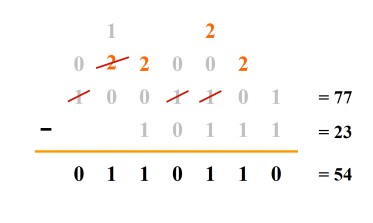
\includegraphics[width=250pt]{img/e1.jpg}}
	\caption{مثالی از تفریق در مبنای دو}
	\label{fig}
\end{figure}

\subsection{جمع و تفریق اعداد علامت دار}
به روش های متداول قبلی قابل انجام است.\\
معمولا در کامپیوتر در سیستم مکمل 2 انجام می شود.\\
بایستی همه عملوند ها را به سیستم مکمل 2 ببریم\\
جواب نهایی در سیستم مکمل 2 بدست خواهد آمد، باید برای خواندن آن دقت کنیم.\\

\subsubsection{جمع دو عدد علامت دار در سیستم مکمل 2}
جمع در سیستم مکمل 2، بدون توجه به مثبت یا منفی بودن اعداد، آنها را زیر هم نوشته و جمع میکنیم، از رقم نقلی خروجی صرف نظر میکنیم یعنی آنرا حذف می کنیم.\\
\textbf{مثال: حاصل عملیات جمع را در 4 بیت در سیستم مکمل دو حساب کنید:}\\
نکته ای که در این مسئله باید به آن توجه داشته باشید، آن است که در هنگام جمع به صورت بی علامت پیش میرویم، برای بررسی هر کدام از صورت جمع ها، آن عددی که بیت علامتش 0 است که به صورت دهدهی عادی تبدیل میشود، در غیر این صورت بایستی اول به صورت مکمل 2 نوشته شده و بعد به مبنای 10 تبدیل شود.\\
\begin{enumerate}
	\item
	$(0001)_{2_{(+1)}} + (1001)_{2_{(-7)}} = (1010)_{2_{-(6)}}$\\
	\item
	$(0010)_{2_{(+2)}} + (0111)_{2_{(7)_{2+7=9}}} = (1001)_{2_{-(0111\rightarrow -7)}}$\\
در مثال بالا در حقیقت Overflow رخ داده که جواب اشتبا بدست آمده است. و فلگ کری 1 خواهد شد چرا که یک بیت اضافی دارد.\\
	\item
	$(0011)_{2_{(+3)}} + (0100)_{2_{(+4)_{+3+4=7}}} = (0111)_{2_{+(7)}}$\\
	\item
$(1001)_{2_{(-7)}} + (0111)_{2_{(+7)_{7-7=0}}} = ([1]0000)_{2_{(0)}}$\\
در مثال بالا، [1] به این خاطر حذف شده چرا که حاصل بدست آمده بیشتر از 4 بیت میشد.\\
\end{enumerate}

\textbf{نکته:}\\
در هنگام جمع دو عدد در مبنای دو، اگر برای مثال صورت اول و صورت دوم هر دو مثبت باشند و در نهایت در نتیجه عددی منفی را داشته باشیم، اورفلو رخ خواهد داد، برای تصحیح این مشکل فقط کافیه است که از روش Extended Sign استفاده کنیم، که اگر 4 بیتی باشد می شود، هشت بیت، اگر هشت بیتی باشد میشود 16 بیت الی آخر. این طور می توان به جواب درست دست پیدا کرد(تکرار عدد اخر).\\
برای مثال، در تمرین دوم بالا، ما اورفلو داریم چرا که نتیجه بدست آمده با جمع کلی درست نیست، یا اینطور جمع دو عدد مثبت باید مثبت شود اما نتیجه منفی شده است، برای بدست آوردن نتیجه درست از Extended Sign استفاده کنیم:\\
$(0000,0010)_{2} + (0000,0111)_{2} = (0000,1001)_{2}$\\
در بالا بیت علامت صفر، اورو فلو صفر، فلگ صفر، صفر و کری هم صفر خواهد بود، و نتیجه بدست امده هم مثبت.


\subsection{Overflow سرریز}
اعداد در کامپیوتر با طول محدود و تعداد بیت های مشخص به کاربرده می شوند.اگر نیتجه محاسبات خارج از این محدوده شود و بیت های بیشتر در دسترس نبایشد، این بیت های اضافی حذف خواهند شد و نتیجه بدست آمده صحیح نخواهد بود. در این حالت می گوییم در انجام محاسبه سرریز اتفاق افتاده است.\\
فلگ v  یا of
$:(Overflow flag)$
این فلگ وقتی 1 میشود که از نتیجه محاسبات در بازه مجاز تعداد بیت نباشد، در این حالت میگوییم اورفلو یا سرریز رخ داده است.\\
در ادامه مطالب حتما مثال هایی در این خصوص زده خواهد شد.

\subsection{بازه مختلف ساخت اعداد در سیستم های مختلف با کمک n بیت}
\raggedleft
در سیستم بی علامت:\\
\raggedright
$0  -  (111...1)_{2} = 2^{n}-1$\\
\raggedleft
در سیستم علامت و مقدار:\\
\raggedright
$(111...1)_{2} = -(2^{n-1}-1) - (111...1)_{2} = (2^{n-1}-1)$\\
\raggedleft
سیستم مکمل یک:\\
\raggedright
$(111...1)_{2} = -(2^{n-1}-1) - (111...1)_{2} = (2^{n-1}-1)$\\
\raggedleft
سیستم مکمل دو:\\
\raggedright
$(111...1)_{2} = -(2^{n-1}) - (111...1)_{2} = (2^{n-1}-1)$\\
\raggedleft

\justifying
\subsection{تشخیص سرریز دو عدد بدون علامت}
در جمع اعداد در سیستم بدون علامت، اگر پس از جمع دو علامت رقم، رقم اخر (نقلی و نهایی) یک شود، سرریز اتفاق خواهد افتاد.\\
$(1101)_{2} + (1100)_{2} = ([1](1001))_{2}$\\

\subsection{تشخیص سرریز در اعداد علامت دار مکمل 2}
\textbf{نکته:}\\
اگه جمع دو عدد منفی، مثبت شود یا جمع دو عدد مثبت منفی شود، سرریز رخ میدهد. دقت داشته باشید، جمع دو عدد مثبت و منفی باهم، سرریز ندارد.\\

اگر دو عدد A و B در سیستم مکمل 1 و 2 باشند، آنگاه A+B در صورتی سرریز خواهد بود که:\\
\begin{enumerate}
	\item
		اگر A و B هر دو مثبت باشند و نتیجه منفی را بدهند.
	\item
	اگر A و B منفی باشند و نتیجه مثبت را بدهند.
\end{enumerate}

\textbf{نتیجه:}\\
اگر دو عدد با علامت های مختلفی داشته باشیم هیچگاه اورفلو رخ نخواهد داد.\\

اگر دو عدد A و B در سیستم مکمل 1 یا 2 باشند، آنگاه A-B در صورتی سرریز خواهد بود که:\\
\begin{enumerate}
	\item
	A
	مثبت باشد و B منفی باشد، و حاصل آنها منفی شود.\\
	درستش:\\
	$(A_{+})-(B_{-})=(+)$
	\item
A
منفی باشد و B عددی مثبت، حاصل آن مثبت شود\\
درستش:\\
	$(A_{-})-(B_{+})=(-)$
\end{enumerate}
دیگر نکته بر روی دیگر فلگ های سادست که مختصرا بیان میکنیم:\\
فلگ zero زمانی 1 میشود که حاصل بدست آمده برابر با صفر باشد در غیر این صورت 0 خواهد بود.\\
فلگ carry زمانی 1 میشود که بیت اضافی وجود داشته باشد.\\
فلگ sign زمانی یک میشود که بیت علامت ما منفی باشد.\\
فلگ اورفلو زمانی یک میشود که حاصل بدست آمده با جمع منطقی ما (اگر عدد صورت اول منفی بود به مکمل 2 میبریم در غیر این صورت بصورت ساده جمع را انجام میدهیم) برابر نباشد.(با توجه به قوانینی که در بالاتر توضیح داده شد)\\
\textbf{حل چند تمرین:}\\

\begin{enumerate}\raggedright
	\item
	$(1001)_{2_{2c(-7)}} + (0111)_{2_{7}} = ([1] 0000)_{2_{(0)}}$\\
	carry = 1, Zero = 1, Of = 0, sign =0
	\item
	$(1101)_{2_{2c=(-3)}} + (1110)_{2_{2c=(-2)}} = ([1] 1011)_{2_{2c=(-5)}}$\\
	carry = 1, Zero = 0, Of = 0, sign =1
	
	\item
	$(0101)_{2_{(5)}} + (0100)_{2_{4}} = (1001)_{2_{2c=(0111 =>-7)}}$\\
	carry = 0, Zero = 0, Of = 1, sign =1

	\item
	$(1001)_{2_{2c=(-7)}} + (1010)_{2_2c={-6}} = ([1] 0011)_{2_{(3)}}$\\
	carry = 1, Zero = 0, Of = 1, sign =0
\end{enumerate}
\begin{figure}[htbp]
	\centerline{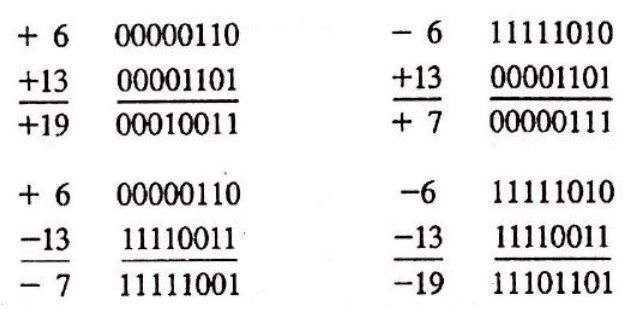
\includegraphics[width=250pt]{img/te1.jpg}}
	\caption{تمرین از جمع اعداد در سیستم مکمل 2}
	\label{fig}
\end{figure}

\subsection{تفریق دو عدد علاممت دار در سیستم مکمل 2}

در هنگام تفریق دو عدد در مکمل 2، میتوانیم عدد A را با مکمل عدد B جمع کنیم. و این جمع مانند جمعی است که در بالاتر توضیح داده شد.
\textbf{حل چند تمرین:}\\

\begin{enumerate}\raggedright
	\item
	$(1101)_{2} - (1001)_{2} \rightarrow (1101)_{2_{2c=(-3)}} + (0111)_{7} =([1] 0100)_{2} $\\
	carry = 1, Zero = 0, Of = 0, sign =0

	\item
	$(1100)_{2} - (1010)_{2} \rightarrow (1100)_{2_{2c=(-4)}} + (0110)_{6} =([1] 0010)_{2} $\\
	carry = 1, Zero = 0, Of = 0, sign =0
	
	\item
	$(1001)_{2} - (0100)_{2} \rightarrow (1001)_{2_{2c=(-7)}} + (1100)_{2c(-4)} =([1] 0101)_{2} $\\
	carry = 1, Zero = 0, Of = 1, sign =0

\end{enumerate}


\textbf{مثال:}\\
با فرض دو عدد دودویی
x = 1010100
و
Y = 1000011
تفریق های زیر را انجام دهید.\\

\begin{enumerate}\raggedright
	\item
	$X - Y$\\
	حل:\\
	$(1010100)_{2} - (1000011)_{2} \rightarrow (1010100)_{2_{2c(-44)}} + (0111101)_{2_{61}}=([1]0010001)_{2_{17}}$\\
		carry = 1, Zero = 0, Of = 0, sign =0
	\item
	$Y - X$
	حل:\\
	$(1000011)_{2} - (1010100)_{2} \rightarrow (1000011)_{2_{2c(-61)}} + (0101100)_{2_{44}}=(1101111)_{2_{-17}}$\\
		carry = 0, Zero = 0, Of = 0, sign =1
\end{enumerate}

پس در هنگام تفریق دو عدد
$A - B$
خواهیم داشت:\\
اگر
$A > B$
پس عددی مثبت خواهیم داشت، و فلگ سر ریز با فلگ علامت صفر خواهد بود.\\
اگر
$A < B$، 
پس عددی منفی خواهیم داشت که هم فلگ علامت و هم فلگ اورفلو 1 خوهد بود.\\
اگر
$A = B$،
در این صورت هر دو یکسان هستند پس جواب صفر را خواهیم داشت که فلگ Zero روشن خواهد شد.




\subsection{سیستم D2B}
این نوع اعداد به زبان خودمانی، فقط در نقش مبنای دو ظاهر می شوند وگرنه از نظر ماهیتی همان اعداد Decimal هستند، این اعداد زمانی مورد استفاده قرار میگیرند که برای تبدیل اعداد Decimal به آنها جایگاه اعداد برایمان مهم نیست، بلکه معنا و مفهوم آن عدد برایمان مهم است، مثلا شما شماره دانشجویی یا یک شماره تلفن یک منطقه را در نظر بگیرید، که هر کدام از اعداد نشان دهنده و به معنای خاصی هست، این اعداد هیچ لزومی ندارد که صرفا دودویی باشند، برای تبدیل اعداد Decimal به اعداد Arithmetic به چهار بیت به ازای هر عدد نیاز است، مانند تبدیل اعداد سیستم ${Hex}$. این اعداد قابل درک هستند، نسبت به اعداد باینری فضای بیشتری را میگیرند و اصلا برای محاسبات جمع و تفریق مناسب نیستند!
\subsubsection{کد کردن اعداد دهدهی}

\begin{itemize}\raggedleft
	\item
کدهای باید به صورت دودویی باشند، زیرا در کامپیوتر همه چیز صفر و یک است.
	\item
کدها فقط نماد یا سمبل نمایش اطلاعات را عوض میکنند و نه مفهوم آن ها را.
	\item
یک کد دودویی n بیت،
$2^{n}$
ترکیب ممکن از یک ها و صفرها را داراست.
\end{itemize}


کد ها به دو دسته تقسیم می شوند:\\
کدهای وزن دار: به هر مکان یک وزن اختصاص داده می شود مثل کد BCD، که دارای وزن
$8 4 2 1$
است.\\
کد های بدون وزن: مثل کد افزودنی 3، که میتوانیم با اضافه کردن 3 عدد به کد BCD به کد Excess-3 رسید.\\
\begin{figure}[htbp]
	\centerline{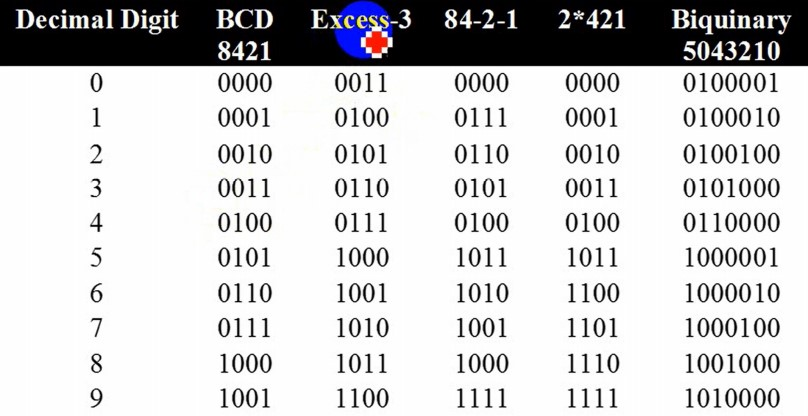
\includegraphics[width=250pt]{img/codes.jpg}}
	\caption{سایر کد های Decimal}
	\label{fig}
\end{figure}

در سیستم کد،
$\overline{1}$
$\overline{2}$
$4$
،$8$
شما می توانید طبق وزن ها از کد BCD به کد مورد نظر خود برسید.\\

در سیستم کد، 2421
از صفر تا 4، وزنمان را از سمت راست تعیین میکنیم، اما از خود پنج به بعد از سمت چپ به عنوان تعیین وزن استفاده خواهیم کرد.\\

\textbf{مثال}\\
عدد
$(82)_{10}$
را به صورت، مبنای 2،
BCD
Excess-3،
،
$\overline{1}$
$\overline{2}$
$4$
$8$،
2421، 
کد کنید.\\

\begin{enumerate}\raggedright
	\item
	$(82)_{10\rightarrow2} = (1010010)_{2}$
	\item
	$(82)_{10} = (1000,0010)_{BCD}$
	\item
	$(82)_{10} = (1000,0010)_{BCD\rightarrow (excess-3)+3} = (1011,0101)_{Excess-3}$
	\item
	$(82)_{10} = (1000,0010)_{BCD \rightarrow 84\overline{2}\overline{1}} = (1000,0110)_{84\overline{2}\overline{1}}$
	\item
	$(82)_{10} = (1000,0010)_{BCD \rightarrow 2421} = (1110,0010)_{2421}$
\end{enumerate}



عدد
$(10111001)_{2}$
را به صورت، مبنای 10،
BCD
Excess-3،
،
$\overline{1}$
$\overline{2}$
$4$
$8$،
2421، 
کد کنید.\\

\begin{enumerate}\raggedright
	\item
	$(10111001)_{2\rightarrow10} = (185)_{10}$
	\item
	$(185)_{10} = (0001,1000,0101)_{BCD}$
	\item
	$(185)_{10} = (0001,1000,0101)_{BCD\rightarrow (excess-3)+3} = (0100,1011,1000)_{Excess-3}$
	\item
	$(185)_{10} =(0111,1000,1011)_{84\overline{2}\overline{1}}$
	\item
	$(185)_{10} = (0001,1110,1011)_{2421}$
\end{enumerate}


\raggedleft
عدد دودویی ${2}_(10111001)$ را به صورت BCD بازنویسی کنید.\\
\raggedright
$(10111001)_{2} = (185)_{10} = (0001,1000,0101)_{BCD}$\\
\raggedleft

\justifying
\subsubsection{جمع دوعدد BCD}
برای جمع اعداد BCD فقط کافیه است که معادل Decimal آنها را با هم جمع کنیم و بعد از آن حاصل را به BCD تبدیل خواهیم کرد.\\
 
\subsection{کد گری یا کد انعکاسی}
زمانی پیش می آید که عدد ورودی ما مثلا
$0111$
که در مبنای 10 برابر با هفت است به عنوان ورودی وارد شده و مثلا میخواد بشود 8 یا $1000$ در طی این تبدیل ممکن است تاخیر ها و Delay های پیش آمده باعث شود به این تبدیل چندین بیت با هم تفاوت و فاصله ایجاد شود، این باعث میشود که CPU زحمت زیادی بکشد در فرایند های تبدیل، به همین خاطر سیستم عددی به نام Gray به وجود آمد که در اثر بوجود آمدن این Delay ها فاصله بین هر عدد تنها یک بیت باشد، کد گری میتواند یک ست 2 بیتی، 3 بیتی 4 بیتی، 5بیتی و غیره باشد، که همه این ها با هم تنها یک بیت فاصله دارند، منظور از یک بیت فاصله یعنی بعد از تبدیل عدد اصلی از حالت بومی خودش به کد گری فقط و فقط یک بیت تفاوت است.\\


 برای تبدیل کد باینری به کد گری خیلی راحت میتوانیم از طریق شباهت و تفاوت پیش برویم، عددی که بیشترین ارزش را دارد (اولین عدد از سمت چپ) یا عدد MSB را بدون هیچ دستکاری می نویسیم، بعد از آن خود آن عدد را با عدد کناری خودش بررسی میکنیم، اگر بایکدیگر مشابه بودند، عدد صفر را مینویسیم، اگر باهم تفاوت داشتند عدد یک را مینویسیم. همین فرایند را تا انتها پیش میرویم. برای مثال:\\
\raggedright
$Same = 0$\\
$Difference = 1$\\
$(110111)_{2\rightarrow Gray} = (101100)_{Gray}$\\

$(111)_{2\rightarrow Gray} = (100)_{Gray}$ \\

$(10101101)_{2\rightarrow Gray} = (11111011)_{Gray}$ \\

 \raggedleft
 \subsubsection{تبدیل باینری 4 بیتی به گری 4 بیت}
\center
\begin{LTR}
	\begin{tabular}{ c | c }
		Binary & Gray\\
		\hline
		0000 & 0000\\
		0001 & 0001\\
		0010 & 0011\\
		0011 & 0010\\
		0100 & 0110\\
		0101 & 0111\\
		0110 & 0101\\
		0111 & 0100\\
		1000 & 1100\\
		1001 & 1101\\
		1010 & 1111\\
		1011 & 1110\\
		1100 & 1010\\
		1101 & 1011\\
		1110 & 1001\\
		1111 & 1000\\	
	\end{tabular}\\
\end{LTR}
\raggedleft

 \subsubsection{تبدیل کد گری به کد باینری}
برای تبدیل کد گری به باینری میباست عدد MSB را نوشته (همانطوری) و بعد از همان به بعد با اعداد بعدی مقایسه میشود\\

\raggedright
$Same = 0$\\
$Difference = 1$\\
$(101100)_{Gragy\rightarrow 2} = (110111)_{2}$\\

$(100)_{Gragy\rightarrow 2} = (111)_{2}$ \\

$(11111011)_{Gragy\rightarrow 2} = (10101101)_{2}$ \\

\begin{figure}[htbp]\centering
	\centerline{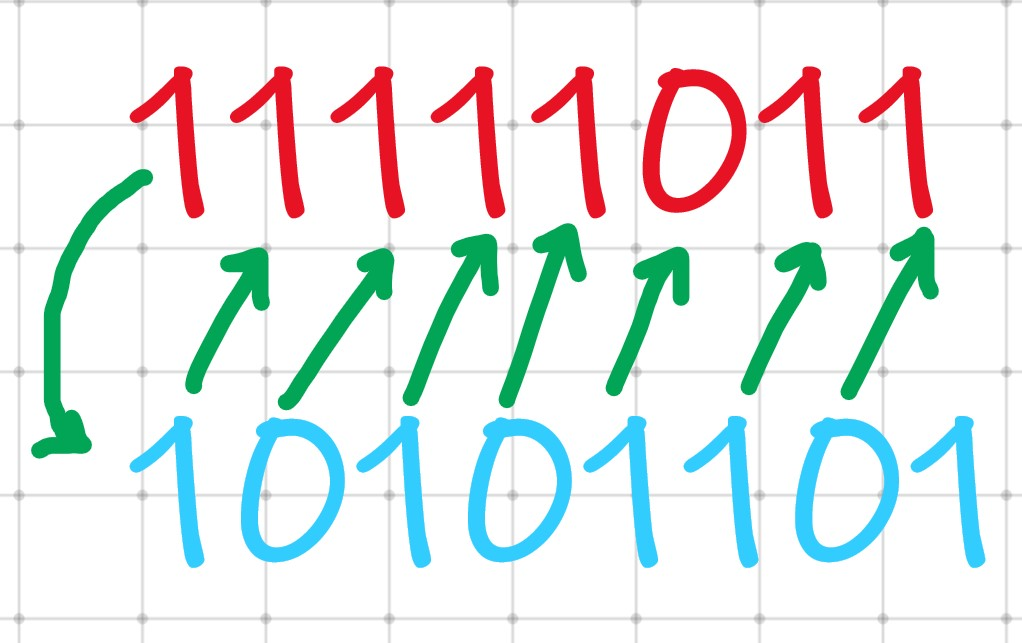
\includegraphics[width=150pt]{img/Gary2Binary.jpg}}
	\caption{Binary 2 Gray}
	\label{fig}
\end{figure}

\raggedleft
\justifying
\subsection{Codes ASCII}
از کدهای اسکلی زمانی استفاده میشود که ما بخواهیم نماد ها، کارکتر های مختلف، اعداد، نماد های زبان های مختلف و غیره را در سیستم خود نمایش بدهیم. این سیستم کدینگ در حالت کلی 8 بیتی میباشد. در 50 سال گذشته این سیستم 6 بیتی بوده و توانایی نمایش حروف فقط بزرگ انگلیسی را داشت، اما بعد از آنکه این سیستم 8 بیتی شد توانایی هایی که در بالاتر توضیح داده شد را دارا میباشند، در این سیستم کدینگ 3 بیت به عنوان ستون ها و 4 بیت به عنوان سطر ها مورد استفاده قرار گرفته، و بیت اخر که بیت مشخص کنند ماهیت کارکتر میباشد، اگر وضعیت این بیت 0 باشد توانایی نمایش اعداد، کارکتر های کنترلی و یکسری علائم و نماد های مختلف مانند
$(` Back Text)$،
:،
;،
"،
را دارای میباشد که به این دسته ها
ASCKII Standard
گفته میشود، که \textbf{تعداد کرکتر های آن 128 تا }می باشد. اما اگر این بیت هشتم 1 باشد علاوه بر نمایش حروف انگلیسی میتواند حروف اضافه بر زبان انگلیسی را نمایش دهد مانند $ü$ در زبان ترکی و آلمانی (اوملات) و غیره. که این دسته در حقیقت ASCKII Extended نامیده میشود، که این دسته هم \textbf{دارای 128 تا کرکتر} میباشد.\\
دسته بندی های کدهای الفبایی یا بطور کلی $Textual$:\\

\raggedright
A ... Z and a...z Alphabet:\\
1..9 Digits:\\
., :, ;, ", `  Symbols Special:\\
DEL, NULL non-printable:\\
\raggedleft
\justifying

\begin{figure}[htbp]
	\centerline{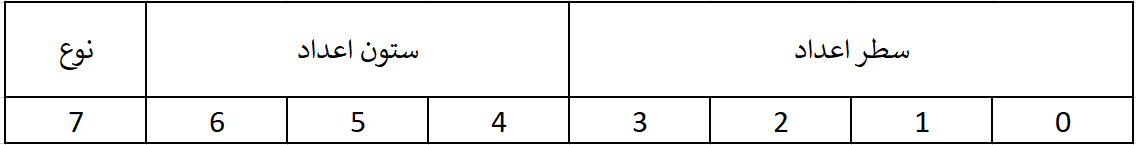
\includegraphics[width=250pt]{img/asciibits.png}}
	\caption{بیت های کد اسکی}
	\label{fig}
\end{figure}

\begin{figure}[htbp]
	\centerline{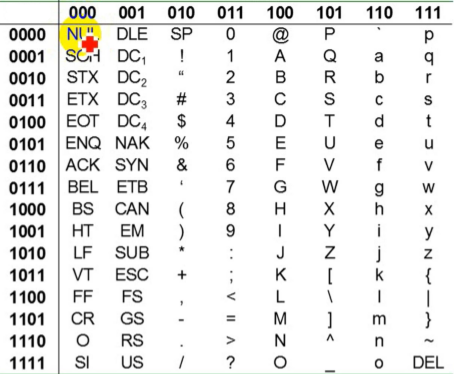
\includegraphics[width=125pt]{img/asciitable.png}}
	\caption{Table Codes ASCII}
	\label{fig}
\end{figure}
مهم ترین بخش جدول کدهای اسکی مربوط به ستون اول و دوم و ابتدای ستون سوم، مربوط به کارکتر های کنترلی میشود، حالا این کاراکتر های کترلی چیست این مهم است:\\
در گذشته ماشین های تله تایپی وجود داشتند که نهایت سرعت آنها 10 بیت در ثانیه بود و کلا یکسری دستگاه های مکانیکالی بودند. این دستگاه های برای ارتبط با سیستم های دیگر از یکسری کرکتر ها استفاده میکردند تا بعضی از جریان ها مورد بررسی قرار بگیرد، برای مثال وقتی به این سیستم ها قرار بود یکسری کلمات و جلملات را بنویسند ارتباط آنها مانند ارتباط ما با کامپیوتر های امروزی نبود و با تاخیری کلمات چاپ میشدند، این سیستم ها برای اینکه ببینند آیا سیستم مکانیکی توانسته کراکتر های قبلی را بنویسد که کارکتر های بعدی را ارسال کند، یا اینکه دست نگهدارد که آن سیستم مکانیکی کار قبلی اش را تمام و سپس بروی کار جدید برود، در این میان از مجموعه ای از کارکتر های کنترلی استفاده میکردند که کنترل جریان را هدایت می نمودند. بطور کلی حفظ کردن نام برخی از آنها دشوار میباشد به همین دلیل در سیستم های امروزی از کنترل ترکیبی بجای استفاده از آن کرکتر ها استفاده کردند، برای مثال کرکتر ESC معادل
$ctrl + [$
است.\\

\raggedleft
\justifying
برای بدست اوردن نام و کلا تایپ این نوع کرکتر ها باید دقت داشته باشیم که از سمت چپ اعداد خود را قرار بدهیم،\textbf{ اولین دسته عدد که سه بیتی} است ستون را منظور دارد، \textbf{دومین دسته که چهار بیتی} است بعد از سه بیت ستون نوشته شده و قرار میگیرد و در انتها برای اینکه بررسی کنیم آیا این عدد یک Extended است یا Standard از سمت چپ بیت MSB را یکی اکستند میکنیم که تا نوع آن مشخص و 8 بیتی شود. و بعد در انتها میتوانیم کد بانری بدست آمده را به دسیمال تبدیل کرده و معادل آن عدد را در کد اسکی بررسی کنیم. مانند:\\

\raggedright
$1100111 \rightarrow (110,111)_{(2) \rightarrow 10} = 103 ~ g$\\

\raggedleft
\begin{figure}[htbp]
	\centerline{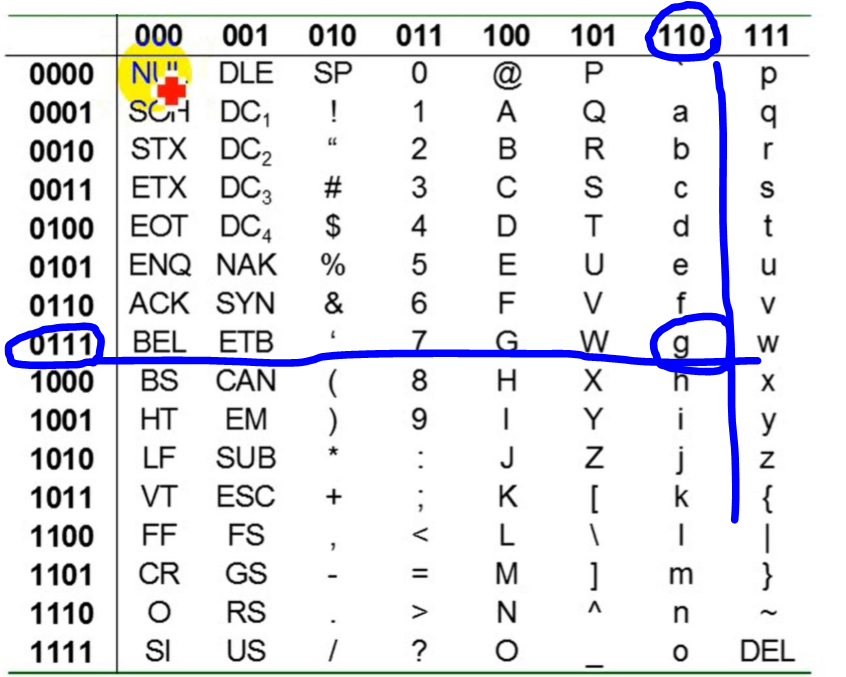
\includegraphics[width=100pt]{img/sampleAsciicode.png}}
	\caption{Sample Codes ASCII}
	\label{fig}
\end{figure}
\justifying
یا اینکه میتوانیم بطور کلی اینگونه پیش برویم که 3 بیت اول از ستون و 4 بیت دوم از سطر جدول را نقطه یابی کنیم که معادل چه حرفی میشود. تصویر بالا\\

\raggedleft
\justifying
\subsection{کد های تشخیص و تصحیح خطا}
هنگام انتقال داده ها ممکن است در آنها خطایی به علت تداخل های الکترومغناطیسی، حرارت زیاد و غیره به وجود آید. میتوان کد هایی طراحی کرد که خطا را تشخیص و تحصیح کنند.\\
یکی از ساده ترین روش های تشخیص خطا استفاده از بیت توازن یا \textbf{Parity} است. میتوان به هر کلمه یک بیت اضافه کرد به طوری که تعداد بیت های یک آن مثلا فرد شود

\subsubsection{کدهای تشخیص خطا}
\justifying
سیستم توازن، يکي از ساده ترین روش ها برای تشخیص خطاست، که یک بیت توازن به اطلاعات اضافه می شود.\\
در حالت کلی دو نوع توازن وجود دارد، توازن زوج و توازن فرد.\\
\raggedleft
\textbf{توازن زوج Parity Even}\\
یک بیت به اطلاعات اضافه میشود تا تعداد کل 1 ها کد زوج جود.\\
\raggedright
$0110010 = [1]0110010 $\\
$0100100 = [0]0100100 $\\
\raggedleft
\textbf{توازن فرد Parity Odd}\\
\raggedright
$0110011 = [1]0110011 $\\
$0100101 = [0]0100101 $\\
\raggedleft
یک بیت به اطلاعات اضافه میشود تا تعداد کل 1 های کد فرد شود. تا تعداد صفر ها و یک ها به تعادل و برابری برسد.\\

\raggedleft
\justifying
نوع دیگری از Parityها وجود دارد که به تعداد یک ها توجه می شود، یعنی اگر سیستم پریتی زوج بودیم تعداد یک ها بایستی زوج باشند، اما اگر در سیستم پریتی فرد بودیم باید تعداد یک ها یک دسته فرد باشند، برای اینکار در سیستم پریتی زوج تعداد یک ها اگر فرد بود یک، 1 را اضافه خواهیم کرد اما اگر زوج بود 0 را وارد میکنیم. در فرد هم همینگونست اگر سیستم فرد تا 1 داشت 0 اگر سیستم زوج تا 1 داشت یک، 1 اضافه میکنیم تا نظم زوجی یک ها را بهم بزنیم و آنها را فرد کنیم!\\

\raggedright
$Even Parity: 100011 = 1 \rightarrow 1000111$\\
$Odd  Parity: 100011 = 0 \rightarrow 1000110$\\

\raggedleft
\justifying
\subsection{Parity Block or Parity Overlapping}
یک مجموعه ای از دیتا ها که بایستی به دو صورت افقی و عمودی از آنها پریتی گرفته شود.\\

\begin{figure}[htbp]
	\centerline{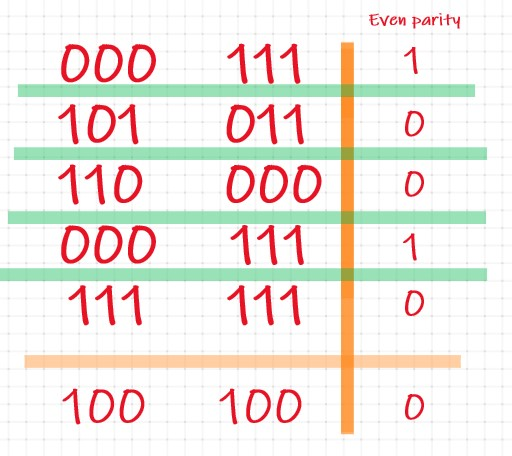
\includegraphics[width=100pt]{img/blockParity.jpg}}
	\caption{Parity Block}
	\label{fig}
\end{figure}

در صورتی که در یکی از بیت های مجموعه داده های بالا خطایی ایجاد شود میتوان براحتی دریافت که در آن قسمت، هم به صورت افقی و هم به صورت عمودی نتیجه پریتی با نتیجه قبلی برابر نخواهد بود. و برای نشان داده اشتباه در آن متقطه باید به صورت یک آرایه دو بعدی طور عمل کنیم که بعد اول در مورد سطر و بعد دوم در مورد ستون میباشد، مانند اشکال در
$M_{[5][3]}$
.

\subsection{Checksum Parity}
در این نوع پریتی ما سه نوع داریم:\\
\subsubsection{checksum Single-precision}
در این نوع از checksum دیتا های دریافتی را با هم جمع میکنیم، و حاصل بدست آمده اگر همراه با Carry بود از آن صرف نظر خواهیم کرد.
\subsubsection{checksum Double-precision}
در این نوع، علاوه بر اینکه کری را به همراه حاصل مینویسیم بایستی بررسی کنیم که وجود کری آیا دسته بیت ها را در توانی از دو قرار داده است یا خیر، اگر نبود خودمان دستی این کار را انجام میدهیم
\subsubsection{checksum Residue}
در این نوع از checksum، مانند Single-precision عمل میکنیم با این تفاوت که کری بدست آمده را در حاصل جمع میکنیم
\subsubsection{checksum HoneyWell}
در این در صورتی که 4 عدد دیتا را داشته باشیم دو به دو دسته ها را بهم می چسبانیم.\\

\begin{figure}[htbp]
	\centerline{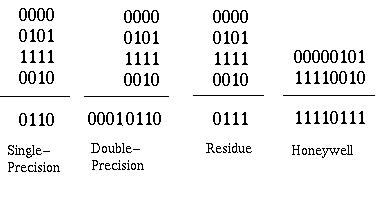
\includegraphics[width=250pt]{img/checksumTypes.jpg}}
	\caption{checksum Parity}
	\label{fig}
\end{figure}



\justifying
\subsection{کد همینگ یا Code Hamming}
بطور کلی، کد همینگ، کد تشخیص و تصحیح خطا می باشد. که در مخابرات مورد استفاده قرار میگیرد. منظور از مخابرات یعنی ارسال و دریافت اطالاعات بین دو قسمت مبدا و مقصد است. که برای اولین بار به افتخار ریچارد همینگ معرفی شد. در مفهوم، در کد همینگ برای شناسایی و تصحیح خطا دسته ای از کد ها در اطلاعات ارسال میشود، که به این کدها کد همینگ می گویند.
\subsubsection{فاصله همینگ}
زمانی که ما کد تحصیح شده را در کنار کدی با بیت های غلط قرار می دهیم به اختلاف بین این دو عدد، فاصله همینگ گفته می شود.\\
\raggedright
$A = 111001 \rightarrow Correct$ \\
$A_{uncorrect} = 010110 \rightarrow uncorrect \rightarrow distance = 5$ \\
\justifying
\textbf{نکته:}\\
\begin{itemize}
	\item
	کدی که فاصله d دارد میتواند $d-1$  خطا را تشخیص دهد.
	\item
کدی که فاصله d دارد میتواند
$\lfloor\frac{d-1}{2}\rfloor$
را تحصیح کند.
\end{itemize}

\justifying
\subsubsection{نحوه بدست همینگ کد و تشخیص  و تصحیح خطا}
برای بدست آوردن کد همینگ یک عدد میبایستی به شکل زیر عمل کنیم:
\begin{itemize}
	\item	
اول باید بررسی کنیم که اعداد دریافت شده چند بیتی است، (تشخیص از تعداد ارقام عدد ارسالی)
	\item
بعد از بدست آوردن تعداد ارقام عدد ارسالی، از سمت چپ باید کد هایی تحت عنوان Parity Code را در نظر داشته باشیم، هر کدام از این کدهای Parity توانی از دو خواهند بود. یعنی\\
$2^{0}, 2^{1}, 2^{2} Or 1, 2, 4, 8,16, 32, etc$
	\item
	باتوجه به قاعده بالا، از سمت چپ جایگاه های مثلا 1 و 2 و 4 و 8 و غیره را برای کد های Parity نگه میداریم، و اعداد داده اصلی را لا به لای این اعداد Parity خواهیم نوشت!

\end{itemize}
\textbf{
با یک مثال نحوه بدست آوردن کد همینگ را متوجه خواهید شد:}\\

کد همینگ برای عدد 0101 به چه شکل خواهد بود؟\\
\begin{figure}[htbp]
	\centerline{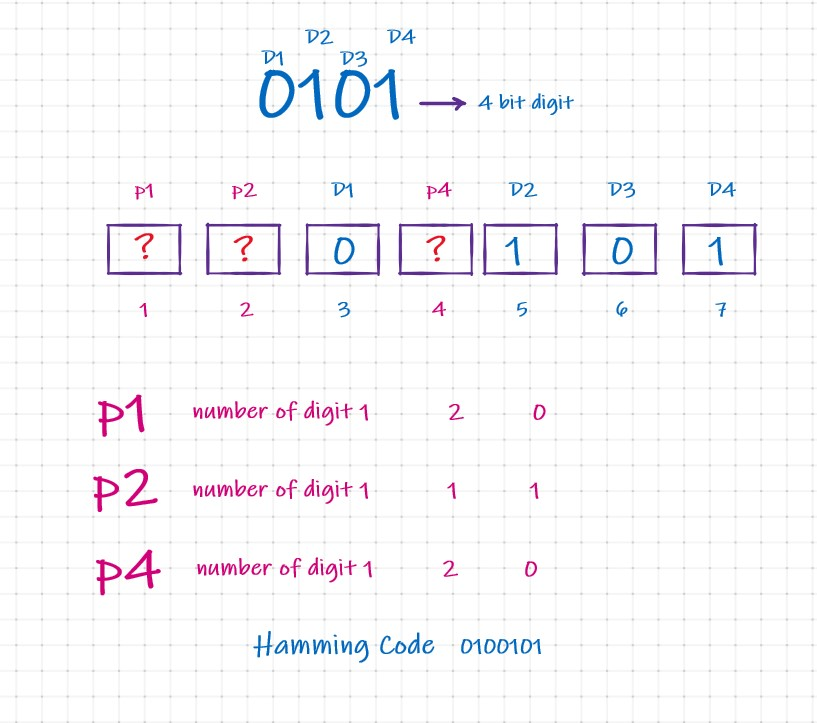
\includegraphics[width=250pt]{img/hamming1.jpg}}
	\caption{مثال بدست آوردن کد همینگ}
	\label{fig}
\end{figure}

توضیح حل مثال بالا:\\
در این مثال ما چهار بیت داریم، و کدهای parity 1 و 2 و4 خواهیم داشت، با توجه به هر عدد بلاک های خالی برای قسمت های 1 و 2 و 4 خواهیم گذاشت تا با روشی مناسب اعداد مناسب آنها را بدست بیاوریم و در قسمت های خالی یا بین این پریتی ها دیتای اصلی خود را خواهیم گذاشت، بعد از تنظیم تمام جایگاه ها و قرار دادن اعداد اصلی در جایگاه مناسب خودشان، با روشی ساده میتوان اعداد پریتی را بدست آورد، اینکه شما میتوانید از جایگاه اول که 1 است یک در میان اعداد 1 و 0 را در نظر بگیرید، صفرها مهم نیستند بلکه باید تعداد یک ها را داشته باشیم، \textbf{اگر }تعداد یک ها \textbf{زوج }بود آن پرتی 0 خواهد بود اگر\textbf{ فرد} بود 1 می باشد، بعد از جایگاه اول به جایگاه دوم یعنی 2 میریم، که میبایست همان کار اول را از دو، با تفاوت 2 در میان انجام دهیم تا مقدار صفر یا یک آن را بدست بیاوریم. بعد به جایگاه چهارم میرویم و بایستی از عدد جایگاه 4، 4 در میان تعداد یک ها را مورد بررسی قرار دهیم.\\

\textbf{نکته:}
گاهی ممکن است به 8 در میان  یا بیشتر از آن، هم برخورد کنید، اگر در انتها به اندازه مناسب n در میان، عددی وجود نداشته باشد، همان تعدادی که وجود دارند را میتوان به عنوان دسته آخر مورد بررسی قرار داد.

\textbf{مثال:}\\
کد همینگ برای عدد 10011010 به چه شکل خواهد بود؟\\
\begin{figure}[htbp]
	\centerline{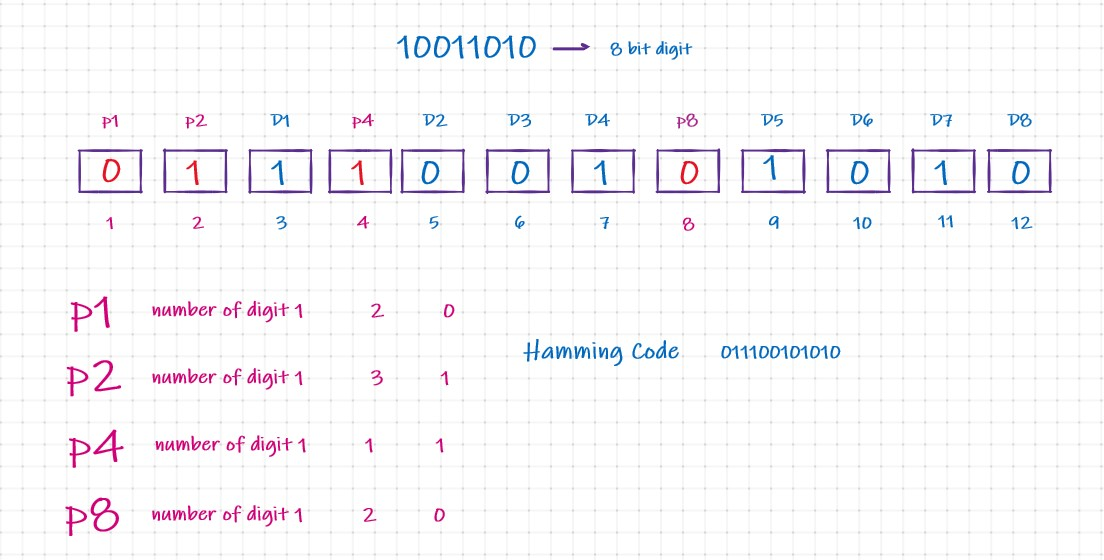
\includegraphics[width=250pt]{img/h2.jpg}}
	\caption{مثال بدست آوردن کد همینگ}
	\label{fig}
\end{figure}

\subsubsection{پیدا کردن عدد غلط و تصحیح آن}
\textbf{نکته دیگری هم هست!
}

ممکن است عددی را به شما دهند که یا اشتباه است یا درست، که شما بایستی با عمل همینگ درستی یا نادرستی آن عدد ارسالی را بررسی کنید.\\

\textbf{مثال:}\\
در عدد 0110101 مشخص کنید که کجا خطا رخ داده است؟\\
در این مثال دیگر کاری به اضافه کردن جایگاه نداشته باشید با این فرض پیش بروید که تمام جایگاه ها همانی است که میدانید:\\
$0_{p1}1_{p2}10_{4}101$\\
$p1 : number of 1: 3 \rightarrow 1$\\
$p2 : number of 1: 2 \rightarrow 0$\\ 
$p4 : number of 1: 2 \rightarrow 0$\\
با توجه فرایندی که در بالا صورت گرفت میتوان نیتجه گرفت که پریتی های بدست آمده با عدد نوشته شده مسئله در جایگاه های مناسب، یا درست است یا غلط، که مشخص کردیم که جایگاه اول و دوم غلط نوشته شده، این موضوغ غلط بودن این عدد را نشان نمیدهد، برای بدست اوردن اشکال در عدد بایستی جایگاه اعداد غلط مانند جایگاه یک و دو را باهم جمع کنیم که می شود 3، آنگاه از این نتیجه میتوان دریافت که در جایگاه سوم عدد درستی درج نشده، اگر صفر است آنرا یک میکنیم، اگر یک است آنرا صفر میکنیم. نکته ای که لازم است در انتها به آن اشاره کنم آن است که در هنگام شمارش تعداد یک های، اگر جایگاهی از خودش یک داشت آنرا حساب نخواهیم کرد.\\
عدد درست، 0100101\\
\textbf{مثال:}\\
عدد 011100101110 درست دریافت شده یا غلط؟ در صورت تشخیص بیت اشتباه آنرا مشخص کنید:\\
$0_{p1}1_{p2}11_{p4}0010_{p8}1110$\\
$p1 : number of 1: 4 \rightarrow 0 Correct$\\
$p2 : number of 1: 4 \rightarrow 0 Uncorrect$\\
$p4 : number of 1: 1 \rightarrow 1 Correct$\\
$p8 : number of 1: 3 \rightarrow 1 Uncorrect$\\
جایگاه های غلط را باهم جمع میکنیم تا جایگاهی که واقعا بیت اشتباهی دارد را تشخیص دهیم، جایگاه 2 با 8 که میشود 10:\\
$0111001011_{_{uncorrect bit}}10$\\
عدد درست
011100101010\\


\subsubsection{نحوه محاسبه تعداد پرتی های همینگ}
یک فرمول ساده در این رابطه وجود دارد
$2^{r} -1 >= (n)bit number + r$
که در آن رقم توان، تعداد پرتی ها و در مقابل تعداد ارقام عدد دریافتی + آن تعداد پرتی\\

برای مثال عدد دودویی داریم که 11 بیت است برای پیدا کردن این که این رقم چند تا جایگاه پرتی خواهد داشت به صورت زیر خواهد بود:\\
$2^{3} - 1 >= 11 + 3 false$\\
$2^{4} - 1 >= 11 + 4 true$\\
پس در 11 بیت 4 بیت پرتی خواهیم داشت.\\

\newpage

\raggedleft
\justifying
\section{جبر بول - ساده سازی - PI, EPI}
اساس کار مدار منطقی، جبر بول یا جبر مجموعه ها یا جبر سویچ است. جبر بول به خاطر آقای Boole George نام گذاری شده است، که برای بیان منطق انسان از آن استفاده نمود. بعد از مدتی Shannonn جبر کلیدی یا Algebra Switching را برای نمایش مدارهای کلیدی دو حالتی معرفی کرد یعنی جبر دو ارزشی.

\subsection{table truth And Or Not }
\center
\begin{LTR}
\begin{tabular}{ c c | c | c | c}
	A & B & A . B & A + B & !A \\
	\hline
	0 & 0 & 0 & 0 & 1\\ 				
	1 & 0 & 0 & 1 & 0\\
	0 & 1 & 0 & 1 & 1\\
	1 & 1 & 1 & 1 & 0\\
\end{tabular}
\end{LTR}

\raggedleft
\justifying
\subsection{استفاده از نمودار وِن برای نمایش منطقی}
ما میتوانیم از نمودار وِن برای نمایش وضعیت های true و false یا 0 و 1 استفاده کنیم.


\subsubsection{Variable Single}

\begin{figure}[htbp]
	\centerline{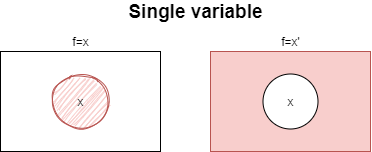
\includegraphics[width=150pt]{img/venn/venn-single variable.png}}
\end{figure}

\subsubsection{Variable Double}

\begin{figure}[htbp]
	\centerline{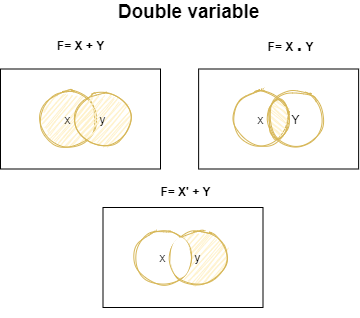
\includegraphics[width=150pt]{img/venn/venn-double Variable.png}}
\end{figure}
\newpage
\subsubsection{Variable Three}

\begin{figure}[htbp]
	\centerline{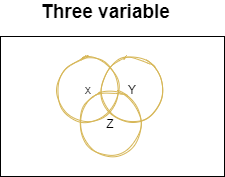
\includegraphics[width=125pt]{img/venn/venn-three_variable.png}}
\end{figure}
جدول زیر نشان دهنده وضعیت سه متغیر، $(X, Y, Z)$ است، هر کدام از وضعیت ها را در وِن نمایش دهید.

\center 
\begin{LTR}
	\begin{tabular}{ c c c }
		X & Y & Z \\
		\hline
		0 & 0 & 0 \\ 				
		0 & 0 & 1 \\
		0 & 1 & 0 \\
		0 & 1 & 1 \\
		1 & 0 & 0 \\
		1 & 0 & 1 \\
		1 & 1 & 0 \\
		1 & 1 & 1 \\	
	\end{tabular}
\end{LTR}

\begin{figure}[htbp]
	\centerline{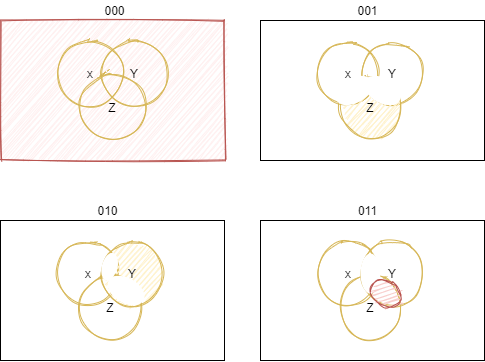
\includegraphics[width=250pt]{img/venn/solution1.png}}
\end{figure}

\begin{figure}[htbp]
	\centerline{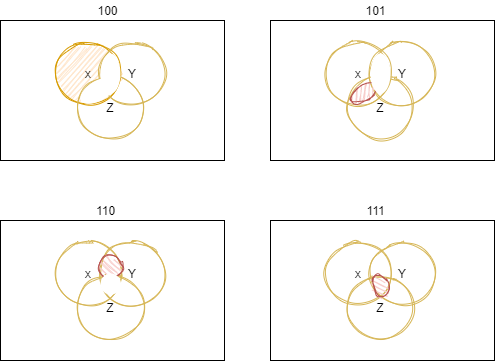
\includegraphics[width=250pt]{img/venn/solution2.png}}
\end{figure}
\newpage

\raggedleft
\justifying
\subsection{off-set and on-set}
به جدول زیر توجه کنید:
\center 
\begin{LTR}
	\begin{tabular}{ c | c c c | c | c }
		Bit Pattern & X & Y & Z & Prime no. & status \\
		\hline
		0 & 0 & 0 & 0 & 0 & off-set \\ 				
		1 & 0 & 0 & 1 & 0 & off-set\\
		2 & 0 & 1 & 0 & 1 & on-set\\
		3 & 0 & 1 & 1 & 1 & on-set\\
		4 & 1 & 0 & 0 & 0 & off-set\\
		5 & 1 & 0 & 1 & 1 & on-set\\
		6 & 1 & 1 & 0 & 0 & off-set\\
		7 & 1 & 1 & 1 & 1 & on-set\\	
	\end{tabular}
\end{LTR}
\hfill \break


\raggedleft
\justifying
جدول بالا در قسمت نتیجه، مشخص میکند عدد در هر سطر اول است یا نه، به هر سطری که مقدر عدد اول بودن آن، برابر با صفر شده است
off-set
و به هر سطری که اول بودن آن یک شده است
on-set
گفته میشود.

% TODO sosis 

% TOD0 multiple input function
\newpage

\subsection{شمایل گیت های تاکنون گفته شده}
\begin{figure}[htbp]
	\centerline{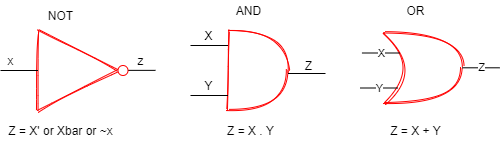
\includegraphics[width=250pt]{img/gates.png}}
\end{figure}

\raggedleft
\justifying

\newpage
\raggedleft
\justifying
\subsection{table truth NAND NOR Xor XNOR }
\center
\begin{LTR}
\begin{tabular}{ c c | c | c | c | c}
	A & B & NAND $\uparrow$ & NOR $\downarrow$ & XOR $\oplus $ & XNOR $\odot$\\
	\hline
	0 & 0 & 1 & 1 & 0 & 1\\ 				
	1 & 0 & 1 & 0 & 1 & 0\\
	0 & 1 & 1 & 0 & 1 & 0\\
	1 & 1 & 0 & 0 & 0 & 1\\
\end{tabular}
\end{LTR}

\newpage
 
\raggedleft
\justifying
راهی دیگر برای اثبات \textbf{Xor} یا \textbf{Xnor} وجود دارد:\\

\raggedright
$XOR = (\overline{A}.B) + (\overline{B}.A) \equiv (\sim A\wedge B) \vee (A \wedge\sim B) $\\
$XNOR = (A.B) + (\overline{A}.\overline{B}) \equiv (A \wedge B)\vee(\sim A\wedge\sim B)$\\

\raggedleft
\justifying

\subsection{چند مورد از اصطلاحات}

\subsubsection{Term}
به هر يک از Variable ها، Term گفته ميشود.

\subsubsection{Term Product}
به هر کدام از ضرب بین عملوند ها یا and بین عملوند ها
\textbf{ Term Products }گفته میشود.\\
مانند:\\

\raggedright
XY or X'Y\\
Uncorrect:\\
$(XY)'$\\
$(XY) + Z$\\

\raggedleft
\justifying
\subsubsection{Term Sum}
	به هر کدام از جمع بین عملوند ها یا or بین آنها	
\textbf{Term Sum}
گفته میشود.\\

\raggedright
$(X + Y)$\\
Uncorrect:\\
$(X+Y)'$\\
$Z'W + Y$\\

\raggedleft
\justifying
\subsubsection{Term Min}
	به هر \textbf{Term Product} گفته میشود که حداقل یکی از آنها True یا 1 باشند.

\raggedleft
\justifying
\subsubsection{Product of Sum SoP}
	به \textbf{Term Product }هایی که بین آنها عمل جمع یا or اتفاق افتاده است، \textbf{Product of Sum }یا \textbf{SoP} گفته می شود.\\

\begin{equation}
	\overbrace{\underbrace{(\overline{A}.B)_{Products Term}} + (\overline{B}.A)}^{Sum of Products}
\end{equation}

\subsubsection{Sum of Product PoS}
	به هر \textbf{Term Sum} که بین آنها عمل ضرب یا And صورت گرفته بر عکس	 SoP در حقیت PoS یا\textbf{ Sum of Products }گفته می شود\\
\begin{equation}
	\overbrace{\underbrace{(\overline{A}+B)_{Sum Term}} . (\overline{B}+A)}^{Products of Sum}
\end{equation}
نکته:\\

	Term
ها
در این حالت آنها به صورت Literal هستند که هر دوی Term Sum و Term Product را شامل می شوند.

\newpage

\subsubsection{خودت را امتحان کن}
\center
\begin{LTR}
	\begin{tabular}{ c | c}
		Expression & Sum Term / Product Term / Both / Neither \\
		\hline
		$W*X*(Y*Z)'$ & Neither\\
		$W*X*(Y*Z)$ & Product Term\\
		$W+XY+Z$ & Neither\\
		$W+Y$ & Sum Term\\
		$(W+Y+Z)'$ & Neither\\
		$W$ & Both\\
	\end{tabular}

\end{LTR}

\raggedleft
\justifying
\subsection{Low Dual}
در قانون دوئال در Term Product ها چند چیز تغییر خواهد کرد:\\

\raggedright
$A.B \leftrightarrow A+B$\\
$0 \leftrightarrow 1$

\raggedleft
\justifying
\textbf{برای مثال:}\\

\raggedright
$f(a.b) \rightarrow f^{*} = a+b$\\
$f = a.1 + \overline{b}.c \rightarrow f^{*}=(a+0) . (\overline{b}+c) $\\
$f()= A \oplus B = (\overline{A}.B) + (A.\overline{B}) \rightarrow f^{*}()= (\overline{A}+B) . (A+\overline{B})$


\raggedleft
\justifying
\subsubsection{Dual Self}
در قانون Dual Self به چیزی اشاره میکند که صحت دوئال آن با حالت عادی آن برابر است\\
برای بررسی تعداد دفعاتی که بایستی true و false یا 0 و 1 بگذاریم، میتوانیم به تعداد عملوندها توجه کنیم و به عنوان توانی از پایه دو استفاده کنیم که ببین چند حالت میتواند این تابع داشته باشد\\
\begin{equation}
	2^{number of Operand}
\end{equation}


\textbf{مثال:}\\
ثابت کنید که تابع
$f=a.b + a.c + b.c$
با هم خود دگان یا سلف دوئال است:\\

\raggedright
$f^{*}() = (a+b).(a+c).(b+c)$

\center
\begin{LTR}
\begin{tabular}{ c c c | c | c}
	a & b & c & $f()$ & $f^{*}()$\\
	\hline
	0 & 0 & 0 & 0 & 0 \\ 				
	0 & 0 & 1 & 0 & 0\\
	0 & 1 & 0 & 0 & 0\\
	0 & 1 & 1 & 1 & 1\\
	1 & 0 & 0 & 0 & 0\\
	1 & 0 & 1 & 1 & 1\\
	1 & 1 & 0 & 1 & 1\\
	1 & 1 & 1 & 1 & 1\\
\end{tabular}
\end{LTR}
\raggedleft
\justifying

\subsubsection{اصل Duality}
اگر دو تابع با هم سلف دوئال باشند، اگر خاصیتی برای حالت عادی تابع صدق کند برای حالت دوئال آن هم صادق میباشد.\\

\subsection{خاصیت های گزاره ها}


\begin{itemize}\centering
	\item
	خاصیت خودتوانی:\\

$A.A = A$ \\
$A+A = A$
	\item
خاصیت جذبی:\\

$A.(A+B) = A$ \\
$A+(A.B) = A$ \\	
	\item
	خاصیت جذبی:\\

$A.(A+B) = A$ \\
$A+(A.B) = A$ \\
	\item
خاصیت جابجایی:\\

$A.B = B.A$ \\
$A+B = B+A$ \\	
	\item
خاصیت شرکت پذیری:\\

$A.(B.C) = (A.B).C$ \\
$A+(B+C) = (A+B)+C$ \\	
	\item
خاصیت توزیع پذیری:\\
$A.(B+C) = (A.B)+(A.C)$ \\
$A+(B.C) = (A+B).(A+C)$ \\	
	\item
خاصیت نقیض نقیض:\\
$\overline{\overline{A}} = A$  	
	\item
خاصیت متمم:\\
$\overline{A} . A = 0$ \\
$\overline{A} + A = 1$ \\	
	\item
خاصیت همانی:\\
$A.1 = A | A+1 = 1$ \\
$A.0 = 0 | A+0 = A$ \\	
	\item
خاصیت دمورگان:\\
$\overline{(A.B)} = (\overline{A} + \overline{B})$ \\
$\overline{(A+B)} = (\overline{A} . \overline{B})$ \\	
\end{itemize}
\raggedleft
\justifying

\subsection{Gates}
گیت ها میتوانند بیشتر از دو ورودی داشته باشند اما توابع در همه آنها مشابه است.\\
در عملگر And، خروجی ها همه یک هستند در صورتی که ورودی ها 1 باشند.\\
 در عملگر OR، خروجی 1 است در صورتی که یکی از ورودی ها 1 باشد.\\


\center 
\begin{LTR}
	\begin{tabular}{ c c }
			\begin{tabular}{ c c c | c }
		X & Y & Z & F \\
		\hline
		0 & 0 & 0 &  0\\ 				
		0 & 0 & 1 &  0\\
		0 & 1 & 0 &  0\\
		0 & 1 & 1 &  0\\
		1 & 0 & 0 &  0\\
		1 & 0 & 1 &  0\\
		1 & 1 & 0 &  0\\
		1 & 1 & 1 &  1\\	
	\end{tabular}
	
	&
		\begin{tabular}{ c c c | c }
		X & Y & Z & F \\
		\hline
		0 & 0 & 0 &  0\\ 				
		0 & 0 & 1 &  1\\
		0 & 1 & 0 &  1\\
		0 & 1 & 1 &  1\\
		1 & 0 & 0 &  1\\
		1 & 0 & 1 &  1\\
		1 & 1 & 0 &  1\\
		1 & 1 & 1 &  1\\	
	\end{tabular}\\
	\hline
	AND & OR
	\end{tabular}
\end{LTR}
\hfill \break

\raggedleft
\justifying
ممکن است در مسئله ای از شما بخواهند که گیتی را با رسم جدول درستی، بررسی یا Checkers / Decode کنید، به همین خاطر مانند زیر عمل میکنیم.\\

\begin{figure}[htbp]
	\centerline{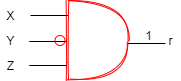
\includegraphics[width=100pt]{img/andGate.png}}
\end{figure}

\raggedleft
\justifying
\newpage
گیت بالا در ورودی دوم، هر مقداری وارد شود نقیض خواهد شد، و از آنجایی که میدانیم، گیت بالا فقط در زمانی جواب 1 را میدهد که تمام ورودی ها یک شوند. به همین خاطر در درون گیت AND هر سه ورودی را یک میکنیم، اما در ورودی های خارج از گیت را باتوجه به نقاط یا حباب هایی که بر روی ورودی گیت کشیده شده، مقادیر مورد نظر را خواهیم نوشت.
\center
\begin{LTR}
	\begin{tabular}{ c c c | c }
		X & Y & Z & F \\
		\hline
		0 & 0 & 0 &  0\\ 				
		0 & 0 & 1 &  0\\
		0 & 1 & 0 &  0\\
		0 & 1 & 1 &  0\\
		1 & 0 & 0 &  0\\
		1 & 0 & 1 &  1\\
		1 & 1 & 0 &  0\\
		1 & 1 & 1 &  0\\	
	\end{tabular}
\end{LTR}
\hfill \break

\begin{figure}[htbp]
	\centerline{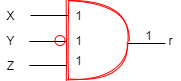
\includegraphics[width=100pt]{img/solAndGate.png}}
\end{figure}

\begin{figure}[htbp]
	\centerline{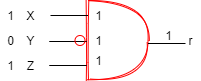
\includegraphics[width=100pt]{img/sol2AndGate.png}}
\end{figure}

\raggedleft
\justifying
پس بخاطر نقیض بودن ابتدا ورودی اول، برای رسیدن به عدد 1، عدد 0 را قرار دادیم که نقیض صفر یک خواهد شد و گیت AND ما در نقطه 101 برابر با یک خواهد بود.\\

مثال دوم:\\

\begin{figure}[htbp]
	\centerline{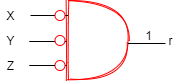
\includegraphics[width=100pt]{img/andGateEmp2.png}}
\end{figure}

\raggedleft
\justifying
جواب:\\

\begin{figure}[htbp]
	\centerline{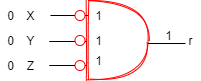
\includegraphics[width=100pt]{img/solAndExmp2.png}}
\end{figure}

\center
\begin{LTR}
	\begin{tabular}{ c c c | c }
		X & Y & Z & F \\
		\hline
		0 & 0 & 0 &  1\\ 				
		0 & 0 & 1 &  0\\
		0 & 1 & 0 &  0\\
		0 & 1 & 1 &  0\\
		1 & 0 & 0 &  0\\
		1 & 0 & 1 &  0\\
		1 & 1 & 0 &  0\\
		1 & 1 & 1 &  0\\	
	\end{tabular}
\end{LTR}
\hfill \break

\raggedleft
\justifying

سه راه برای نمایش یک تابع وجود دارد:
\begin{LTR}
\begin{itemize}
	\item
	Equation 
	\item
	Schematic 
	\item
	Truth table $\rightarrow$ unique
\end{itemize}
\end{LTR}

که حالت جدول درستی معیار است چرا که تنها یک معنا دارد و از آن میتوان به روش های دیگر رسید و آنها را پیاده سازی نمود.\\


\textbf{مسئله:}\\
ماشینی داریم که خودکار است، اگر در ورودی آن و چراغ های جلو روشن باشد، بوق میزند یا اگر در ورودی آن باز باشد و سویچ (کلید) روی حالت on باشد بازم بوق میزند، تابع این مسئله را بنویسید.
\footnote{
ساده سازی بین هر کدام از Term ها مانند فاکتورگیری در ریاضیات در این قسمت Adjacency گفته میشود
}
\center
\begin{LTR}
	\begin{tabular}{ c c }
		\begin{tabular}{ c c c | c }
		H & D & K & F \\
		\hline
		0 & 0 & 0 &  0\\ 				
		0 & 0 & 1 &  0\\
		0 & 1 & 0 &  0\\
		0 & 1 & 1 &  1\\
		1 & 0 & 0 &  0\\
		1 & 0 & 1 &  0\\
		1 & 1 & 0 &  1\\
		1 & 1 & 1 &  0\\	
	\end{tabular} & 
	
		\begin{tabular}{ c c c | c }
		H & D & K & F \\
		\hline
		0 & 1 & 1 &  1\\
		1 & 1 & 0 &  1\\
	\end{tabular}
	
	\end{tabular}
\end{LTR}
\hfill \break

\begin{equation}
	H.D + D.K or H(D + K)
\end{equation}

\raggedleft
\justifying
بیلی دوست داره که فقط پیزایی با قیمت 5 دلار بخورد! یک پیزای 5 دلاری میتواند فقط یکی از موارد (سوسیس، قارچ، پپرونی) را داشته باشد، اما امروز یه تخفیفی فروشگاه گذاشته که بیلی میتونه پیزای سوسیس و قارچ رو باهم در قیمت 5 دلار داشته باشه، تابع و نمودار درستی این مسئله را بنویسید.\\

\begin{LTR}
	\begin{tabular}{ c c c | c}
		S & M & P & Results\\
		\hline
		0 & 0 & 0 & 1\\
		0 & 0 & 1 & 1\\
		0 & 1 & 0 & 1\\
		0 & 1 & 1 & 0\\
		1 & 0 & 0 & 1\\
		1 & 0 & 1 & 0\\
		1 & 1 & 0 & 1\\
		1 & 1 & 1 & 0\\
	\end{tabular}
\end{LTR}
از آنجایی که معلوم است:\\

\center
\begin{LTR}
	\begin{tabular}{ c c }
		\begin{tabular}{ c c c | c}
			S & M & P & Results\\
			\hline
			0 & 0 & 0 & 1\\
			0 & 0 & 1 & 1\\
			0 & 1 & 0 & 1\\
			1 & 0 & 0 & 1\\
			1 & 1 & 0 & 1\\
		\end{tabular} & 
			\begin{tabular}{ c c c | c | c}
		S & M & P & Boolean Form & Results\\
		\hline
		0 & 0 & 0 & $\bar{S} \bar{M} \bar{P}$ & 1\\
		0 & 0 & 1 & $\bar{S} \bar{M} P$ & 1\\
		0 & 1 & 0 & $\bar{S} M \bar{P}$ & 1\\
		1 & 0 & 0 & $S \bar{M} \bar{P}$& 1\\
		1 & 1 & 0 & $S M \bar{P}$& 1\\
	\end{tabular}
	\end{tabular}
\end{LTR}

\raggedleft
\justifying

\begin{equation}
 W= (\bar{S} \bar{M} \bar{P}) + (\bar{S} \bar{M} P) + (\bar{S} M \bar{P}) + (S \bar{M} \bar{P}) +  (S M \bar{P})
\end{equation}
تابع ساده شده\\
\begin{equation}
 W= P + M + S + (SM)
\end{equation}






\newpage

\raggedleft
\justifying
\subsection{Functions Intermediate}
گاهی اوقات برای بدست اوردن یک نتیجه میتوانیم از یکسری تابع تحت عنوان توابع واسط
\footnote{intermediate}
استفاده کنیم، برای مثال، در مسئله زیر دو تابع واسط بین تابع نهایی G آمده است که ما میتوانیم به کمک آن به نتیجه G برسیم:\\

\center
\begin{LTR}
	\begin{tabular}{ c c }
		\begin{tabular}{ c c c | c | c | c}
			X & Y & Z & F1 & F2 & G\\
			\hline
			0 & 0 & 0 &  0 &  0& 0 \\ 				
			0 & 0 & 1 &  1 &  0& 1 \\
			0 & 1 & 0 &  1 &  0& 1 \\
			0 & 1 & 1 &  1 &  0& 1 \\
			1 & 0 & 0 &  1 &  0& 1 \\
			1 & 0 & 1 &  1 &  0& 1 \\
			1 & 1 & 0 &  1 &  0& 1 \\
			1 & 1 & 1 &  1 &  1& 0 \\	
		\end{tabular}
		
	\end{tabular}
\end{LTR}
\hfill \break
\raggedleft
\justifying
بطورکلی تابع اول، OR بین تمام عملوند ها میباشد، و تابع دوم AND بین آنها، در تابع G در ابتدا شباهت 0 را در دو تابع داریم اما زمانی که دو تابع به عدد 1 رسیده اند، نتیجه G برابر با 0 شده است، برای بدست اوردن تابع G میتوانیم به این صورت عمل کنیم:\\

\begin{figure}[htbp]
	\centerline{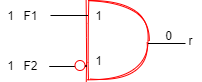
\includegraphics[width=100pt]{img/intermediateExmp.png}}
\end{figure}
\newpage

\raggedleft
\justifying
با توجه به نتايج تابع G با استفاده از توابع Term Min تابع جدول را بدست آورید.
\footnote{
در حقیقت Term Min هایی که در نظر داریم بایستی \textbf{Form Boolean} آن ورودی ها را اول بنویسیم و در قسمت هایی که تابع داده شده حداقل یک بار یک بوده است Term Mid ها بدست خواهد آمد.}

\begin{LTR}
	\begin{tabular}{ c c c | c }		
		X & Y & Z & G \\
		\hline
		  0 & 0  & 0  &1 \\
		  0 & 0  & 1  &1 \\
		  0 & 1  & 0  &0 \\
		  0 & 1  & 1  &0 \\
		  1 & 0  & 0  &1 \\
		  1 & 0  & 1  &0 \\
		  1 & 1  & 0  &1 \\
		  1 & 1  & 1  &0 \\
	\end{tabular}
\end{LTR}
\newpage

جواب:\\
\begin{LTR}
	\begin{tabular}{ c c c | c | c }		
		X & Y & Z & Min Terms\footnote{Boolean Form} & G \\
		\hline
		  0 & 0  & 0  & $\bar{X} \bar{Y} \bar{Z}$  &1 \\
		  0 & 0  & 1  & $\bar{X} \bar{Y} Z$  &1 \\
		  0 & 1  & 0  & $\bar{X} Y \bar{Z}$  &0 \\
		  0 & 1  & 1  & $\bar{X} Y Z$  &0 \\
		  1 & 0  & 0  & $\bar{X} Y Z$  &1 \\
		  1 & 0  & 1  & $X \bar{Y} Z$  &0 \\
		  1 & 1  & 0  & $X Y \bar{Z}$  &1 \\
		  1 & 1  & 1  & $X Y Z$  &0 \\
	\end{tabular}
\end{LTR}

\hfill \break
\begin{LTR}
	\begin{tabular}{ c c c | c | c }		
		X & Y & Z & Min Terms & G \\
		\hline
		  0 & 0  & 0  & $\bar{X} \bar{Y} \bar{Z}$  &1 \\
		  0 & 0  & 1  & $\bar{X} \bar{Y} Z$  &1 \\
		  1 & 0  & 0  & $\bar{X} Y Z$  &1 \\
		  1 & 1  & 0  & $X Y \bar{Z}$  &1 \\
	\end{tabular}
\end{LTR}

\begin{equation}
	W = (\bar{X} \bar{Y} \bar{Z}) +
	(\bar{X} \bar{Y} Z) +
	(\bar{X} Y Z) +
	(X Y \bar{Z})
\end{equation}
\newpage

مثال دوم:\\
\begin{LTR}
	\begin{tabular}{ c c c | c }		
		X & Y & Z & G \\
		\hline
		  0 & 0  & 0  &0 \\
		  0 & 0  & 1  &0 \\
		  0 & 1  & 0  &1 \\
		  0 & 1  & 1  &1 \\
		  1 & 0  & 0  &0 \\
		  1 & 0  & 1  &0 \\
		  1 & 1  & 0  &1 \\
		  1 & 1  & 1  &0 \\
	\end{tabular}
\end{LTR}
جواب:\\
\begin{LTR}
	\begin{tabular}{ c c c | c | c }		
		X & Y & Z & Min Terms & G \\
		\hline
		  0 & 0  & 0  & $\bar{X} \bar{Y} \bar{Z}$  &0 \\
		  0 & 0  & 1  & $\bar{X} \bar{Y} Z$  &0 \\
		  0 & 1  & 0  & $\bar{X} Y \bar{Z}$  &1 \\
		  0 & 1  & 1  & $\bar{X} Y Z$  &1 \\
		  1 & 0  & 0  & $\bar{X} Y Z$  &0 \\
		  1 & 0  & 1  & $X \bar{Y} Z$  &0 \\
		  1 & 1  & 0  & $X Y \bar{Z}$  &1 \\
		  1 & 1  & 1  & $X Y Z$  &0 \\
	\end{tabular}
\end{LTR}
\hfill \break
جا هایی که تابع G ، یک شده است:
\footnote{
جاهایی که تابع داده شده یک شده است در حقیقت مشخص کننده Term Mid هامون هستند که Form Boolean آنها Term Product بین آنهاست
}
\begin{LTR}
	\begin{tabular}{c c c | c | c }		
		X & Y & Z & Min Terms & G \\
		\hline
		  0 & 1  & 0  & $\bar{X} Y \bar{Z}$  &1 \\
		  0 & 1  & 1  & $\bar{X} Y Z$  &1 \\
		  1 & 1  & 0  & $X Y \bar{Z}$  &1 \\
	\end{tabular}
\end{LTR}
\begin{equation}
	W = (\bar{X} Y \bar{Z}) +
	(\bar{X} Y Z) +
	(X Y \bar{Z})
\end{equation}
\newpage














%\section{گیت ها - منطق سه حالته - هازارد - تکنولوژی های ساخت تراشه}

%\section{مدارات ترکیبی}

%\section{لچ ها و فلیپ فلاپ ها}

%\section{تحلیل مدارات ترتیبی سنکرون - میلی و مور - شمارنده ها  و ثبات}

%\section{طراحی مدارات ترتیبی سنکرون - کاهش حالات}

%\section{سنتز مدار با زبان برنامه نویسی وریلاگ}

\end{document}
